% Tarea 3: Introduccion a series de tiempo
% Compilar desde doc/ con:  tectonic -X compile tarea3.tex
% Antes hay que correr los scripts de src/ para generar figuras y tablas.
\documentclass[11pt,letterpaper]{article}

% Con XeTeX (tectonic) se usa fontspec; con T1 el signo de apertura de
% pregunta sale como libra esterlina. Con pdflatex se usa T1 normal.
\usepackage{iftex}
\ifXeTeX
  \usepackage{fontspec}
\else
  \usepackage[utf8]{inputenc}
  \usepackage[T1]{fontenc}
\fi
\usepackage[spanish,es-tabla,es-nodecimaldot]{babel}
\usepackage{amsmath,amssymb,amsthm}
\usepackage{graphicx}
\usepackage{booktabs}
\usepackage{array}
\usepackage{multirow}
% Columna de ancho fijo sin justificar, para que no queden huecos entre palabras
\newcolumntype{L}[1]{>{\raggedright\arraybackslash}p{#1}}
\usepackage[margin=2.4cm]{geometry}
\usepackage{xcolor}
\usepackage[most]{tcolorbox}
\usepackage{enumitem}
\usepackage{caption}
\usepackage{parskip}
\setlength{\parskip}{0.75em plus 0.2em minus 0.1em}

% Los subtitulos de nivel paragraph van numerados y con el texto debajo,
% no corrido en la misma linea.
\setcounter{secnumdepth}{4}
\makeatletter
\renewcommand\paragraph{\@startsection{paragraph}{4}{\z@}%
  {2.6ex \@plus 1ex \@minus .2ex}%
  {1.1ex \@plus .2ex}%
  {\normalfont\normalsize\bfseries}}
\makeatother
\usepackage[hidelinks]{hyperref}

\graphicspath{{../figs/}{figs/}{./}}

% Generado por los scripts de src/.
% No editar a mano: se sobrescribe en cada ejecucion.
\newcommand{\BandaPcero}{0.1132}
\newcommand{\RechazoRuido}{0.0462}
\newcommand{\RechazoRuidoEE}{0.0030}
\newcommand{\RcincoCaminata}{0.881}
\newcommand{\RunoCaminata}{0.975}
\newcommand{\PhiOLSCaminata}{0.9820}
\newcommand{\PhiOLSnueve}{0.8870}
\newcommand{\PhiOLSmedio}{0.4913}
\newcommand{\PhiOLScero}{-0.0022}
\newcommand{\RunoRuido}{-0.0022}
\newcommand{\RechazoTend}{0.987}
\newcommand{\RechazoSem}{0.108}
\newcommand{\RunoTend}{0.247}
\newcommand{\RsieteTend}{0.232}
\newcommand{\RunoSem}{-0.047}
\newcommand{\RsieteSem}{0.265}
\newcommand{\LBdiezRuido}{0.050}
\newcommand{\LBdiezTend}{1.000}
\newcommand{\LBdiezSem}{0.952}
\newcommand{\LBseisSem}{0.212}
\newcommand{\LBQpropio}{33.6542}
\newcommand{\LBQsm}{33.6542}
\newcommand{\LBPpropio}{0.0002}

% Generado por los scripts de src/.
% No editar a mano: se sobrescribe en cada ejecucion.
\newcommand{\FilasCrudas}{541{,}909}
\newcommand{\Facturas}{25{,}900}
\newcommand{\Productos}{4{,}070}
\newcommand{\Clientes}{4{,}372}
\newcommand{\FracSinCliente}{24.9\%}
\newcommand{\FilasLimpias}{531{,}877}
\newcommand{\FilasQuitadas}{10{,}032}
\newcommand{\FracQuitadas}{1.9\%}
\newcommand{\FilasNegSinC}{1{,}336}
\newcommand{\NegSinCConCliente}{0}
\newcommand{\NegSinCPrecioMax}{0}
\newcommand{\FilasCancel}{9{,}288}
\newcommand{\MontoCancel}{-\pounds896{,}812}
\newcommand{\VentaNetaLimpia}{\pounds9{,}697{,}276}
\newcommand{\VentaNetaCruda}{\pounds9{,}747{,}748}

% Generado por los scripts de src/.
% No editar a mano: se sobrescribe en cada ejecucion.
\newcommand{\DiasCalendario}{374}
\newcommand{\DiasAbiertos}{305}
\newcommand{\DiasCerrados}{69}
\newcommand{\SabadosCerrados}{51}
\newcommand{\SabadosAbiertos}{0}
\newcommand{\CerradosNoSabado}{18}
\newcommand{\SinExplicar}{0}
\newcommand{\UltimaHora}{12:50}
\newcommand{\VentaUltimoDia}{\pounds29{,}306}
\newcommand{\FilasUltimoDia}{1{,}618}
\newcommand{\HoraCierreMediana}{17:24}
\newcommand{\VentaViernesPrevios}{\pounds49{,}599}

\newcommand{\NEntrena}{245}
\newcommand{\BandaEntrena}{0.125}
\newcommand{\RezagosFuera}{5}
\newcommand{\RunoReal}{0.210}
\newcommand{\RseisReal}{0.416}
\newcommand{\RdoceReal}{0.277}
\newcommand{\PicoACF}{6}
\newcommand{\QseisReal}{71.4}
\newcommand{\QdoceReal}{96.9}
\newcommand{\PseisReal}{2.1\times 10^{-13}}
\newcommand{\PdoceReal}{2.2\times 10^{-15}}
\newcommand{\PromIndices}{1.200}
\newcommand{\SaltoSeisFrac}{88\%}
\newcommand{\MMEnero}{\libra{}20{,}808}
\newcommand{\MMNoviembre}{\libra{}47{,}057}
\newcommand{\MMMax}{\libra{}54{,}795}

% Generado por los scripts de src/.
% No editar a mano: se sobrescribe en cada ejecucion.
\newcommand{\PhiResiduos}{0.278}
\newcommand{\FueraU}{2, 4, 6, 9}
\newcommand{\ReunoE}{0.276}
\newcommand{\ReseisE}{0.217}
\newcommand{\RedoceE}{0.081}
\newcommand{\RuseisU}{0.161}
\newcommand{\SunoConst}{4.212}
\newcommand{\SunoPhi}{0.132}
\newcommand{\SunoPhiS}{0.521}
\newcommand{\SdosTheta}{-0.914}
\newcommand{\SdosThetaS}{-0.670}
\newcommand{\MediaSuno}{\pounds24{,}878}
\newcommand{\NombresSuno}{intercept, ar.L1, ar.S.L6, sigma2}
\newcommand{\NombresSdos}{ma.L1, ma.S.L6, sigma2}

% Generado por los scripts de src/.
% No editar a mano: se sobrescribe en cada ejecucion.
\newcommand{\NdiasB}{128}
\newcommand{\NdiasC}{58}
\newcommand{\NdiasPrueba}{58}
\newcommand{\NorigenesB}{22}
\newcommand{\NorigenesC}{10}
\newcommand{\ConvSuno}{32 de 32}
\newcommand{\ConvSdos}{32 de 32}
\newcommand{\Ganador}{S2}
\newcommand{\MediaEntrena}{\pounds27{,}632}
\newcommand{\MediaPrueba}{\pounds49{,}768}
\newcommand{\MediaMayoSep}{\pounds29{,}342}
\newcommand{\LagMayo}{\pounds31{,}435.26}
\newcommand{\MAEcB1}{22{,}472}
\newcommand{\MAEcB2}{14{,}409}
\newcommand{\MAEcM1}{15{,}202}
\newcommand{\MAEcM2}{15{,}153}
\newcommand{\MAEcS1}{16{,}739}
\newcommand{\MAEcS2}{12{,}545}
\newcommand{\MAEbB1}{10{,}254}
\newcommand{\MAEbB2}{11{,}341}
\newcommand{\MAEbM1}{9{,}832}
\newcommand{\MAEbM2}{9{,}277}
\newcommand{\MAEbS1}{9{,}657}
\newcommand{\MAEbS2}{10{,}057}
\newcommand{\MAEaB1}{10{,}251}
\newcommand{\MAEaM1}{9{,}150}
\newcommand{\MAEaM2}{8{,}318}
\newcommand{\MAEaTrampa}{7{,}475}
\newcommand{\MAEbTrampa}{8{,}386}

% Generado por los scripts de src/.
% No editar a mano: se sobrescribe en cada ejecucion.
\newcommand{\ClientesRFM}{3{,}615}
\newcommand{\ClientesMneg}{11}
\newcommand{\ClientesSoloCancel}{43}
\newcommand{\FracFuno}{40.1\%}
\newcommand{\FmaxUno}{1}
\newcommand{\FmaxDos}{1}
\newcommand{\FminTres}{1}
\newcommand{\FracCompra}{50.8\%}
\newcommand{\AUCR}{0.672}
\newcommand{\AUCF}{0.720}
\newcommand{\AUCM}{0.709}
\newcommand{\AUCSuma}{0.734}
\newcommand{\NCampeones}{777}
\newcommand{\FracCampeones}{21.5\%}
\newcommand{\VentaCampeones}{53.3\%}
\newcommand{\NNuevos}{721}
\newcommand{\VentaNuevos}{15.7\%}
\newcommand{\VentaOctDic}{\libra{}2{,}400{,}689}


\definecolor{marco}{HTML}{2A7F7A}
\definecolor{fondo}{HTML}{FBF8F3}

\newcommand{\code}[1]{\texttt{#1}}
% Libra esterlina que funciona igual dentro y fuera de modo matematico
\newcommand{\libra}{\text{\pounds}}
% Lee las filas generadas por los scripts dentro de un tabular
\makeatletter\newcommand{\filas}[1]{\@@input #1 }\makeatother
\DeclareMathOperator{\Var}{Var}
\DeclareMathOperator{\Cov}{Cov}
\DeclareMathOperator{\E}{E}

% Caja para las respuestas cortas a cada pregunta
\newtcolorbox{respuesta}{enhanced, breakable, colback=fondo, colframe=marco,
  boxrule=0pt, leftrule=2.5pt, arc=0pt, left=8pt, right=8pt, top=4pt, bottom=4pt}

\title{\textbf{Tarea 3: Introducción a Series de Tiempo}}
\author{Sofía Sandoval\\
        Análisis y Ciencia de Datos\\
        Facultad de Ingeniería, Universidad del Istmo de Guatemala}
\date{\today}

\begin{document}
\maketitle

\begin{abstract}
\noindent
La primera mitad del trabajo simula procesos cuya respuesta se conoce: un
AR(1) con cuatro valores de $\phi$ y dos procesos sin memoria pero con media
cambiante. Con 5\,000 réplicas de cada uno se ve que la prueba de retardo 1
reprueba a una tendencia que no tiene memoria y deja pasar a un patrón
semanal que sí tiene estructura, igual que le pasó a RANDU en la Tarea 2, y
que Ljung--Box con $m=10$ sí lo detecta. La segunda mitad trabaja con las
\FilasCrudas{} líneas de factura de Online Retail. Se documentan cinco reglas
de limpieza en una bitácora, se reconstruye el calendario de la tienda
(cierra los sábados y en los bank holidays, incluida la boda real de 2011) y
se hace una descomposición clásica con media móvil e índices estacionales. La
ACF de la serie tiene su pico en el rezago 6, que es una semana de días
abiertos. Después se pasa del AR(1) a dos SARIMA con $s=6$, y sólo el modelo
con diferencias (S2) deja residuos de ruido blanco. En el pronóstico con
origen móvil semanal, S2 gana en prueba con un MAE de \pounds\MAEcSdos{}, pero
todas las estimaciones hechas dentro del entrenamiento se quedan cortas,
porque la serie casi duplicó su nivel en la temporada navideña. El trabajo
cierra con un análisis RFM: los campeones son el \FracCampeones{} de los
clientes y generan el \VentaCampeones{} de la venta de octubre a diciembre,
y los clientes nuevos aportan un \VentaNuevos{} que ningún modelo cliente por
cliente puede ver.
\end{abstract}

\newpage
\tableofcontents
\newpage

% ===========================================================================
\section{Introducción}

En las tareas anteriores casi todos los datos eran intercambiables: se podían
barajar las filas y nada cambiaba. En una serie de tiempo eso ya no es cierto,
porque el orden es justamente la información. Lo que se vendió ayer dice algo
de lo que se va a vender hoy, los lunes no se parecen a los domingos, y el
futuro no se puede usar para entrenar.

El trabajo está dividido en dos mitades. En la Parte 0 se construye el
vocabulario con procesos simulados: como se conoce el proceso que generó los
datos, se puede comprobar qué ve y qué no ve cada herramienta. La idea central
es que una serie puede reprobar una prueba de independencia por dos razones
muy distintas, porque tiene memoria o porque su media no es constante, y que
distinguir una de la otra es la mitad del trabajo.

En las Partes 1 a 6 se aplica todo eso a datos reales: las transacciones de
un año de una tienda en línea del Reino Unido que vende artículos de regalo,
casi todo a mayoristas. Primero se limpian (Parte 1) y se reconstruye el
calendario (Parte 2). Después se separa la tendencia y la estacionalidad
semanal (Parte 3), se modela la memoria que queda con un AR(1) y con dos
modelos SARIMA (Parte 4), se compara el pronóstico de seis modelos con tres
formas distintas de validar (Parte 5) y, al final, se mira a los clientes que
hay detrás de la serie con un análisis RFM (Parte 6).

Todos los números, tablas y figuras de este documento los generan los scripts
de \code{src/} a partir del archivo \code{Online Retail.xlsx} original, con
las semillas que se documentan en el README.

% ===========================================================================
\section{Apoyo de inteligencia artificial}

Para la elaboración de este trabajo se contó con el apoyo de una herramienta
de inteligencia artificial. El proceso fue el siguiente.

Primero se hizo una lectura personal del enunciado y de las secciones
recomendadas de los dos libros de referencia (FPP2 y Tsay), y se definió qué
pedía cada inciso. Esas notas y las fuentes se le compartieron a la
herramienta para que le sirvieran de base.

Para el código se le entregaron las semillas que debían usarse y las
decisiones de limpieza que se habían tomado al revisar los datos. Sobre esa base se le pidió apoyo
para escribir las implementaciones y para darle un estilo propio a las
gráficas.

Los resultados se analizaron de forma personal, y esos análisis se le
entregaron en borrador para que ayudara a mejorar la redacción antes de
incorporarlos al documento. También se le pidió ayuda con el código del
documento en \LaTeX.

Por último se hizo una revisión completa del documento para verificar que
cada cifra coincidiera con lo que producen los scripts y para mejorar la
estructura y las conclusiones.

% ===========================================================================
\newpage
\section{Parte 0: Procesos simulados}

\subsection{Derivaciones a mano (0.1)}

El modelo es $Y_t = c + \phi Y_{t-1} + \varepsilon_t$ con
$\varepsilon_t \overset{iid}{\sim} N(0,\sigma^2)$ y $|\phi|<1$. Se usan dos
hechos: si el proceso es estacionario, $\E[Y_t]=\E[Y_{t-1}]$ y
$\Var(Y_t)=\Var(Y_{t-1})$; y $\varepsilon_t$ es independiente de todo el
pasado, en particular de $Y_{t-1}, Y_{t-2}, \dots$

\paragraph{Media} Tomando valor esperado en ambos lados,
\[
\E[Y_t] = c + \phi\,\E[Y_{t-1}] + \E[\varepsilon_t] = c + \phi\,\E[Y_t]
\quad\Longrightarrow\quad
\E[Y_t]\,(1-\phi) = c
\quad\Longrightarrow\quad
\E[Y_t] = \frac{c}{1-\phi}.
\]
La división es válida porque $|\phi|<1$ implica $\phi\neq 1$.

\paragraph{Varianza} La constante no aporta varianza y, como
$\varepsilon_t$ es independiente de $Y_{t-1}$, la covarianza entre ambos es
cero:
\[
\Var(Y_t) = \phi^2\Var(Y_{t-1}) + \Var(\varepsilon_t) = \phi^2\Var(Y_t) + \sigma^2
\quad\Longrightarrow\quad
\Var(Y_t) = \frac{\sigma^2}{1-\phi^2}.
\]
Aquí hace falta $|\phi|<1$ para que $1-\phi^2>0$ y la varianza sea positiva y
finita.

\paragraph{Autocorrelación} Sea $\mu = c/(1-\phi)$ y
$X_t = Y_t - \mu$. Restando $\mu = c + \phi\mu$ al modelo queda
$X_t = \phi X_{t-1} + \varepsilon_t$. Para $k\ge1$, multiplicando por
$X_{t-k}$ y tomando valor esperado,
\[
\gamma_k = \E[X_t X_{t-k}] = \phi\,\E[X_{t-1}X_{t-k}] + \E[\varepsilon_t X_{t-k}]
= \phi\,\gamma_{k-1} + 0,
\]
porque $X_{t-k}$ sólo depende de choques anteriores a $t$. Aplicando la
recursión $k$ veces, $\gamma_k = \phi^k\gamma_0$, y por lo tanto
\[
\rho_k = \frac{\gamma_k}{\gamma_0} = \phi^k .
\]

\paragraph{Caminata aleatoria} Con $\phi=1$, $c=0$ y $Y_0=0$, al desenrollar
la recursión queda $Y_t = \varepsilon_1 + \varepsilon_2 + \dots + \varepsilon_t$.
Como los choques son independientes, las varianzas se suman:
\[
\Var(Y_t) = \sum_{i=1}^{t}\Var(\varepsilon_i) = t\sigma^2 .
\]
La varianza depende de $t$ y crece sin límite, así que no se cumple la
condición $\Var(Y_t)=\sigma^2$ para todo $t$ de la estacionariedad débil. Es
también lo que hace que la derivación anterior no aplique: con $\phi=1$ la
fórmula $\sigma^2/(1-\phi^2)$ da una división entre cero. Intuitivamente, la
caminata nunca olvida un choque, así que la incertidumbre se acumula.

\subsection{Simulación (0.2)}

Se programó una función que simula $n=300$ pasos de un AR(1) con $c=0$ y
$\sigma=1$, arrancando en $Y_0=0$ y descartando los primeros 200 pasos para
que el valor inicial no importe. Con $|\phi|<1$ eso funciona porque el efecto
de $Y_0$ decae como $\phi^{200}$, que para $\phi=0.9$ ya es del orden de
$10^{-10}$. Con $\phi=1$ no funciona, porque la caminata nunca olvida: el
valor en el paso 200 se arrastra para siempre. Sin embargo, eso no afecta a
$r_k$, porque lo único que deja la quema es un nivel constante $Y_{200}$ que
se suma a toda la serie, y $r_k$ resta la media muestral antes de calcular
nada. Sumar una constante a toda la serie no cambia ni el numerador ni el
denominador de $r_k$.

La figura~\ref{fig:realizaciones} muestra una realización de cada escenario.
Se ve cómo la memoria cambia el aspecto de la serie: con $\phi=0$ no hay
patrón, con $\phi=0.5$ aparecen rachas cortas, con $\phi=0.9$ la serie se
queda varios pasos del mismo lado del cero, y la caminata aleatoria deambula
sin volver a ningún nivel.

\begin{figure}[htbp]\centering
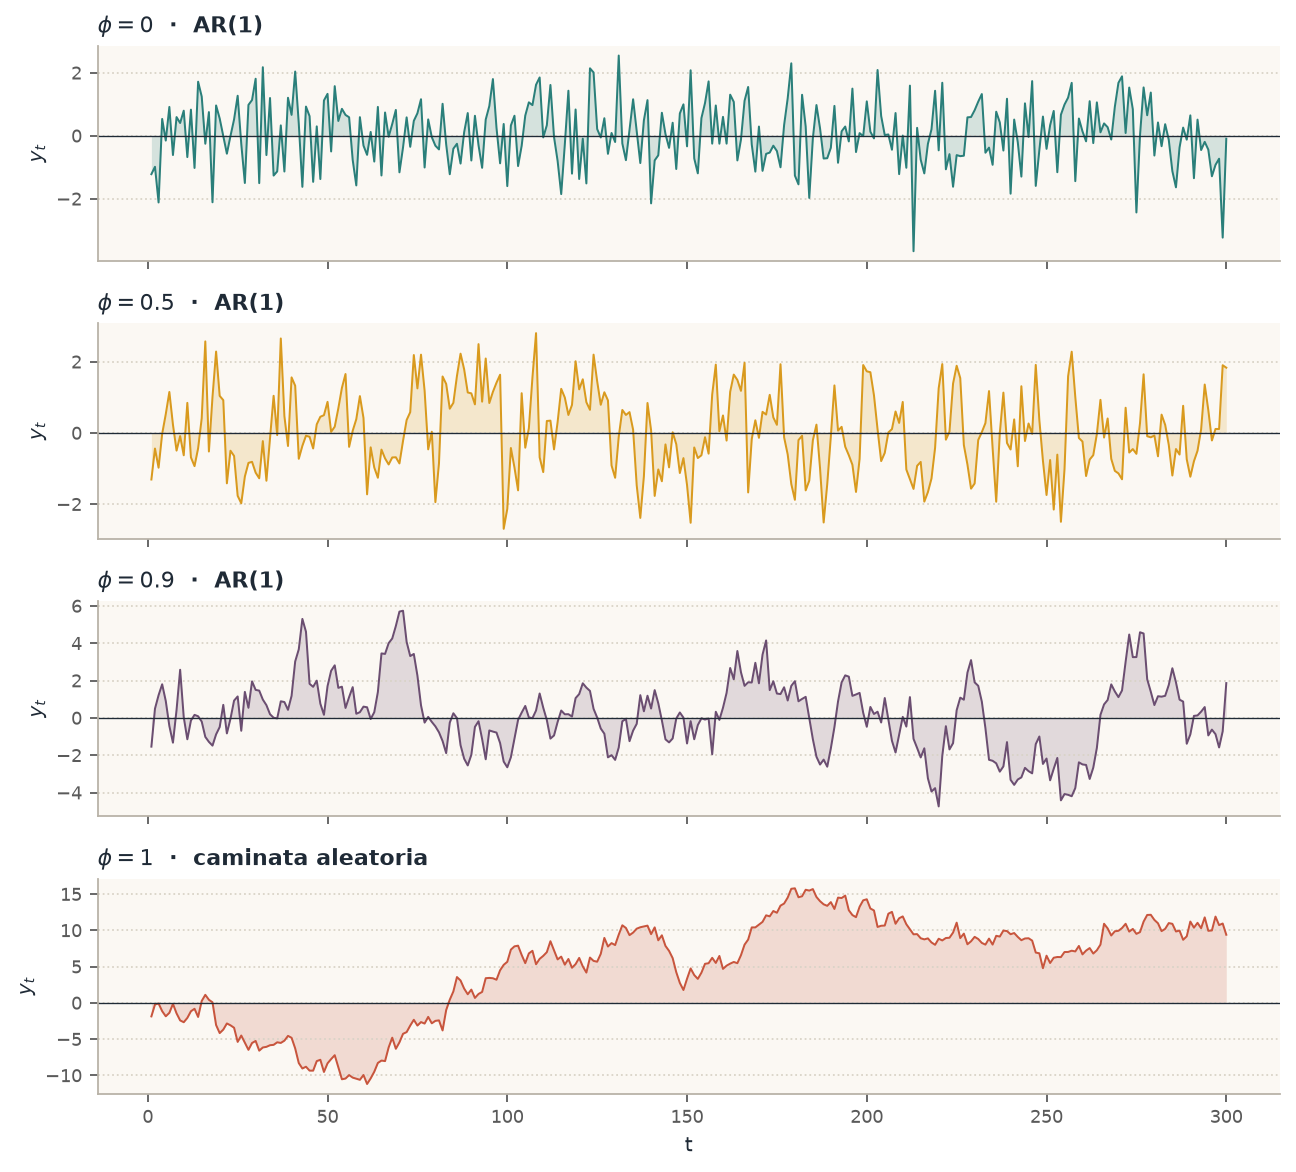
\includegraphics[width=0.88\textwidth]{p0_realizaciones.png}
\caption{Una realización de 300 pasos para cada valor de $\phi$.}
\label{fig:realizaciones}
\end{figure}

Después se hicieron 5\,000 réplicas de cada escenario, con una semilla
distinta para cada $\phi$ (Tabla~\ref{tab:ar1}). Entre paréntesis va el error
estándar de cada promedio, $s/\sqrt{5000}$ para las medias y
$\sqrt{\hat p(1-\hat p)/5000}$ para la tasa de rechazo, que es una proporción.
La banda de la prueba es $1.96/\sqrt{300} = \BandaPcero$.

\begin{table}[htbp]\centering\small
\caption{AR(1) con 5\,000 réplicas por escenario. Entre paréntesis, el error
estándar del promedio.}
\label{tab:ar1}
\begin{tabular}{@{}c rr rr r rr rr@{}}
\toprule
$\phi$ & \multicolumn{2}{c}{$\bar r_1$} & \multicolumn{2}{c}{$\bar r_5$} &
$\phi^5$ & \multicolumn{2}{c}{Rechazo $|r_1|>1.96/\sqrt n$} &
\multicolumn{2}{c}{$\bar{\hat\phi}_{\text{OLS}}$} \\
\midrule
\filas{tabla_p0_ar1}
\bottomrule
\end{tabular}
\end{table}

\subsection{Lectura de la tabla (0.3)}

\paragraph{La tasa de rechazo con $\phi=0$} Sale $\RechazoRuido$, con un error
estándar de $\RechazoRuidoEE$, así que es compatible con el 5\,\% que se
esperaba: está a menos de dos errores estándar. Es lo que tiene que pasar,
porque con ruido blanco $r_1\approx N(0,1/n)$ y la banda está puesta
justamente para que el 5\,\% de las veces se salga por pura suerte. La
pequeña diferencia hacia abajo se explica porque la aproximación normal es
asintótica: con $n$ finito, $r_1$ tiene un ligero sesgo negativo (su media es
cerca de $-1/n$) y una varianza un poco menor que $1/n$.

\paragraph{La caminata aleatoria y $r_5$} La teoría diría $\phi^5=1$, pero el
promedio de $r_5$ es apenas $\RcincoCaminata$. La fórmula $\rho_k=\phi^k$
supone estacionariedad, y la caminata no lo es: no tiene una media fija
alrededor de la cual oscilar. La media muestral $\bar y$ queda en algún punto
del recorrido de esa realización, y $r_k$ mide qué tanto se parecen los
desvíos respecto a ese punto. Con una serie finita, esos desvíos se ven
menos correlacionados a medida que $k$ crece, aunque el proceso nunca olvide
nada. En otras palabras, $r_k$ estima algo que para la caminata no existe.

\paragraph{El sesgo del OLS} Sí hay sesgo, siempre hacia abajo, y crece con
$\phi$: para $\phi=0.5$ el promedio es $\PhiOLSmedio$, para $\phi=0.9$ es
$\PhiOLSnueve$ y para la caminata $\PhiOLSCaminata$. Con errores estándar de
cuatro diezmilésimas, las tres diferencias son claramente reales. Es el
sesgo clásico de muestra finita del AR(1), que aproximadamente vale
$-(1+3\phi)/n$: con $n=300$ eso predice $-0.008$ y $-0.012$ para $\phi=0.5$ y
$0.9$, muy cerca de lo que se observa. La razón es que el regresor
$y_{t-1}$ no es independiente de los errores pasados, así que el supuesto de
exogeneidad del OLS no se cumple exactamente. El estimador sigue siendo
consistente (el sesgo baja como $1/n$), pero con 300 observaciones todavía
se nota, y es más fuerte cerca de la raíz unitaria.

\subsection{Las dos razones para reprobar (0.4)}

Ahora se simulan procesos sin ninguna memoria, $Y_t = m_t + \varepsilon_t$,
pero con media cambiante: una tendencia lineal $m_t = 2t/300$ y un patrón
semanal donde el día $t \bmod 7 = 6$ vale $-1.5$ y los demás $0.25$. La
Tabla~\ref{tab:media} repite el ejercicio y agrega $r_7$, y la
figura~\ref{fig:media} muestra una realización y la ACF promedio de cada uno.

\begin{table}[htbp]\centering\small
\caption{Procesos sin memoria con media cambiante, 5\,000 réplicas.}
\label{tab:media}
\begin{tabular}{@{}l rr rr rr@{}}
\toprule
Proceso & \multicolumn{2}{c}{$\bar r_1$} & \multicolumn{2}{c}{$\bar r_7$} &
\multicolumn{2}{c}{Rechazo con $r_1$} \\
\midrule
\filas{tabla_p0_media}
\bottomrule
\end{tabular}
\end{table}

\begin{figure}[htbp]\centering
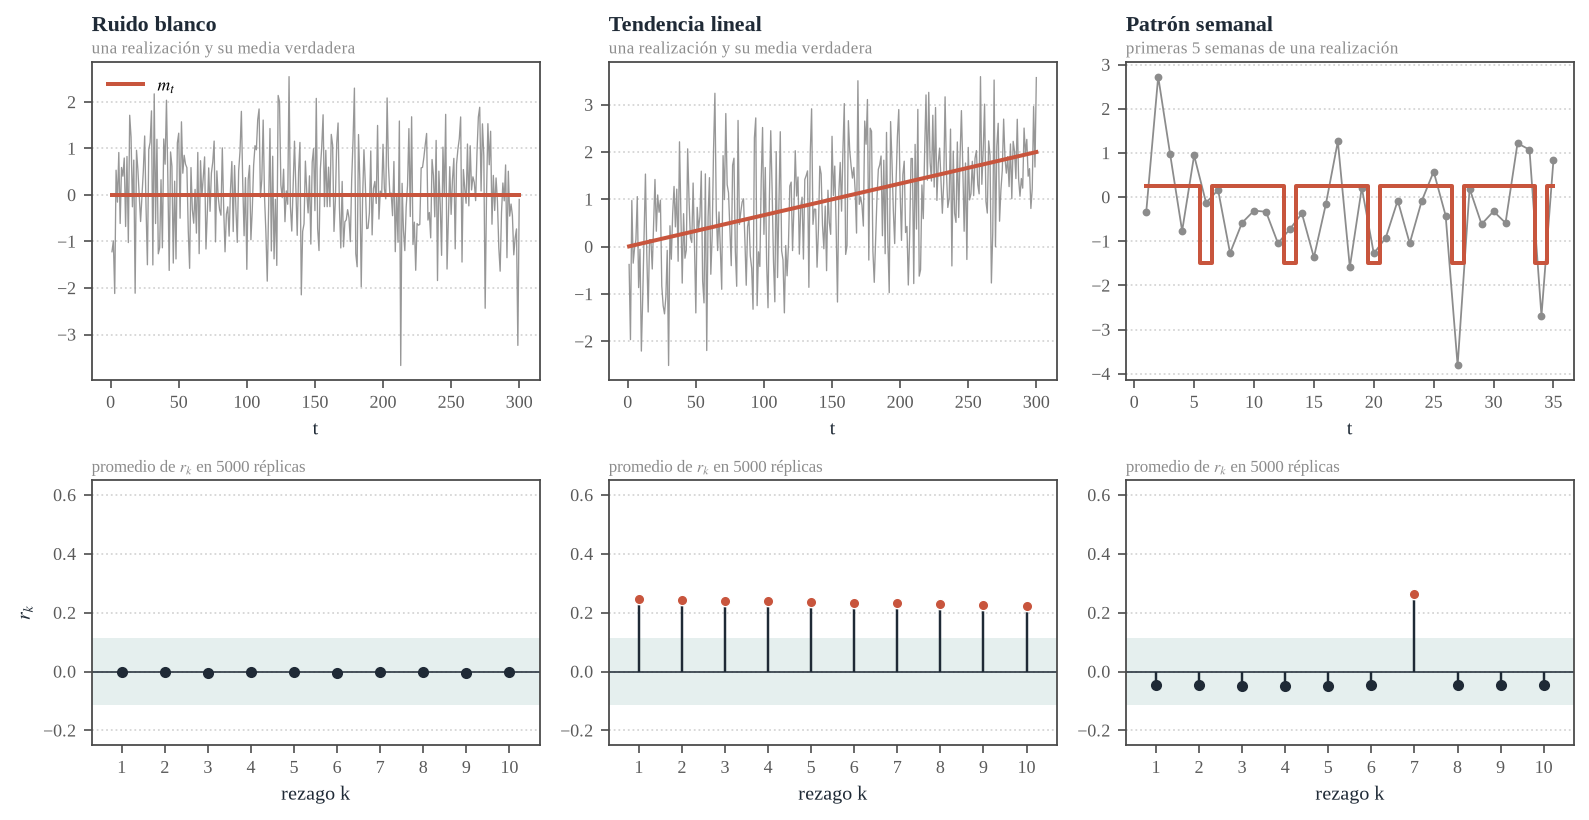
\includegraphics[width=\textwidth]{p0_media_cambiante.png}
\caption{Arriba, una realización de cada proceso con su media verdadera.
Abajo, el promedio de $r_k$ en las 5\,000 réplicas; los puntos terracota se
salen de la banda.}
\label{fig:media}
\end{figure}

\begin{respuesta}
\textbf{La tendencia reprueba sin tener memoria.} Rechaza en el
$\RechazoTend$ de las réplicas, con $\bar r_1 = \RunoTend$. Los días del final
están todos por encima de $\bar y$ y los del principio todos por debajo, así
que cada valor se parece a su vecino aunque los choques sean independientes.
Su ACF es casi plana ($r_7=\RsieteTend$): baja muy despacio, que es la pista
visual de la media no constante.

\textbf{El patrón semanal pasa la prueba aunque tenga estructura.} Sólo
rechaza en el $\RechazoSem$ de las réplicas: $r_1 = \RunoSem$ casi no se
mueve, porque el día bajo está rodeado de días normales. Toda la estructura
está en el rezago 7 ($r_7 = \RsieteSem$), que la prueba de retardo 1 no mira.
\end{respuesta}

La conexión con RANDU es directa. En la Tarea 2, RANDU pasó la prueba de
autocorrelación de retardo 1 sin problema, pero sus ternas consecutivas caían
en 15 planos, porque cumple exactamente
$x_{k+2} = 6x_{k+1} - 9x_k \pmod{2^{31}}$. En los dos casos la dependencia
existe, pero vive en un rezago o en una combinación de rezagos que la prueba
no está mirando. Una prueba que sólo ve un rezago sólo puede confirmar la
ausencia de dependencia en ese rezago, nada más.

\subsection{La prueba que sí ve (0.5)}

Se implementó Ljung--Box a mano con la fórmula del enunciado y se comprobó
contra la función \code{acorr\_ljungbox} de statsmodels: sobre la misma
serie, la implementación propia da $Q(10)=\LBQpropio$ y statsmodels da
$\LBQsm$, idénticos. La Tabla~\ref{tab:lb} compara las tasas de rechazo al
5\,\%. Como pide la sección teórica, se probaron los dos criterios para
elegir $m$: $m=10$ (FPP2 sin estacionalidad) y $m=6\approx\log 300$ (Tsay).

\begin{table}[htbp]\centering\small
\caption{Tasa de rechazo al 5\,\% de la prueba de retardo 1 y de Ljung--Box.}
\label{tab:lb}
\begin{tabular}{@{}l rr rr rr@{}}
\toprule
Proceso & \multicolumn{2}{c}{Retardo 1} & \multicolumn{2}{c}{Ljung--Box $m=6$} &
\multicolumn{2}{c}{Ljung--Box $m=10$} \\
\midrule
\filas{tabla_p0_ljungbox}
\bottomrule
\end{tabular}
\end{table}

Con ruido blanco, Ljung--Box con $m=10$ rechaza el $\LBdiezRuido$ de las
veces, que es exactamente el nivel nominal: no se vuelve más estricta con el
proceso que sí cumple. Con la tendencia rechaza siempre, igual que la prueba
de retardo 1. El cambio está en el patrón semanal: pasa de $\RechazoSem$ a
$\LBdiezSem$. Ljung--Box junta $r_1,\dots,r_{10}$ en un solo estadístico, así
que el $r_7$ grande entra en la suma y la prueba lo ve. Por la misma razón,
con $m=6$ sólo rechaza el $\LBseisSem$: el rezago 7 queda fuera de la suma.
Ésa es la lección práctica sobre cómo elegir $m$: tiene que cubrir el periodo
estacional, y por eso FPP2 recomienda $m=2s$ cuando hay estacionalidad. El
criterio $m\approx\log n$ de Tsay funciona bien sin estacionalidad, pero aquí
se queda corto.

% ===========================================================================
\newpage
\section{Los datos y la Parte 1: Limpieza}

\subsection{Carga y tamaño (1.1)}

Los datos son el archivo \code{Online Retail.xlsx} del repositorio de UCI. Al
cargarlo, las columnas \code{InvoiceNo}, \code{StockCode} y \code{CustomerID}
se leen como texto, por tres razones. \code{InvoiceNo} mezcla números
(\code{536365}) con códigos que empiezan con letra (\code{C536379}), y
leerlos como número rompe la columna o pierde el prefijo, que es justamente lo
que dice si una factura es cancelación. \code{StockCode} también mezcla
códigos numéricos (\code{71053}) con alfanuméricos (\code{85123A},
\code{POST}). Y \code{CustomerID}, como tiene celdas vacías, pandas lo lee
como número decimal (\code{17850.0}), que es un identificador y no una
cantidad: no tiene sentido sumarlo ni promediarlo, y el \code{.0} estorba al
cruzar tablas.

El archivo tiene \FilasCrudas{} filas, \Facturas{} facturas distintas,
\Productos{} códigos de producto y \Clientes{} clientes. El \FracSinCliente{}
de las filas no tiene \code{CustomerID}.

\subsection{Los casos sospechosos (1.2)}

La Tabla~\ref{tab:casos} cuantifica cada caso sobre los datos crudos, cada uno
por separado, y la Tabla~\ref{tab:codigos} desglosa los códigos que no
empiezan con cinco dígitos. La decisión para cada caso es la siguiente.

\begin{table}[htbp]\centering\small
\caption{Cada caso medido sobre los datos crudos, por separado (un mismo
renglón puede estar en más de un caso). El monto es la suma de
\code{Quantity}~$\times$~\code{UnitPrice}.}
\label{tab:casos}
\begin{tabular}{@{}l r r@{}}
\toprule
Caso & Filas & Monto \\
\midrule
\filas{tabla_p1_casos}
\bottomrule
\end{tabular}
\end{table}

\begin{table}[htbp]\centering\small
\caption{Códigos de \code{StockCode} que no empiezan con cinco dígitos.}
\label{tab:codigos}
\begin{tabular}{@{}l L{5.6cm} r r l@{}}
\toprule
Código & Descripción & Filas & Monto & Decisión \\
\midrule
\filas{tabla_p1_codigos}
\bottomrule
\end{tabular}
\end{table}

\paragraph{(a) Filas duplicadas exactas: se van} Hay 5\,268 filas idénticas
en todas las columnas, incluida la hora al minuto. Una misma factura no
debería tener dos líneas iguales del mismo producto en el mismo minuto: es
un registro doble del sistema. Se conserva la primera aparición.

\paragraph{(b) Facturas que no empiezan con un dígito} Hay dos prefijos. Las
\FilasCancel{} líneas con \code{C} son cancelaciones: \textbf{se quedan},
con su cantidad negativa, para que resten el día en que ocurren, como pide el
enunciado. Las 3 líneas con \code{A} son ``Adjust bad debt'': un ajuste
contable por deuda incobrable, no una venta ni una devolución de mercancía.
\textbf{Se van}.

\paragraph{(c) Códigos que no son productos} La pista de la descripción
separa tres grupos. Los cargos de envío (\code{POST}, \code{DOT},
\code{C2}), las comisiones y cargos bancarios (\code{AMAZONFEE},
\code{BANK CHARGES}, \code{CRUK}) y las muestras (\code{S}) \textbf{se van}:
no son venta de mercancía, y algunos ni siquiera son ingresos (la comisión
de Amazon resta \pounds221\,520 en apenas 34 líneas). Los \code{DCGS\ldots},
los vales de regalo \code{gift\_0001\_\ldots} y \code{PADS} \textbf{sí son
productos} y se quedan. El caso intermedio es \code{M} (Manual) y \code{D}
(Discount): no son productos, pero corrigen el precio de ventas reales. La
mayoría de las líneas \code{M} grandes están en facturas \code{C}, y el caso
más claro está en la sección~\ref{sec:top6}: una venta capturada con un
precio 60 veces mayor que se anula con una línea Manual. Si se quitaran las
\code{M}, la venta mal capturada se quedaría sin su corrección. Por eso
\code{M} y \code{D} \textbf{se quedan} como ajustes de la venta neta.

\paragraph{(d) Precios cero o negativos: se van} Con precio cero la línea no
mueve dinero: son regalos, líneas de inventario o errores de captura, y no
aportan nada a la venta. Los dos precios negativos son las líneas de deuda
incobrable de (b).

\paragraph{(e) Cantidades negativas sin C: se van} Las \FilasNegSinC{} líneas
tienen todas precio cero y ninguna tiene cliente. Sus descripciones son
``check'', ``damaged'', ``thrown away'', ``wet pallet'', ``?''\,: son ajustes
de inventario por mercancía dañada o perdida, no devoluciones de clientes. No
mueven dinero.

\paragraph{(f) Filas sin \code{CustomerID}: se quedan para la serie} Son el
\FracSinCliente{} de las filas y \pounds1.45 millones de venta. Para la venta
neta diaria lo que importa es cuánto se vendió, no quién compró, y quitarlas
haría que la serie subestimara sistemáticamente la venta. En la Parte 6 la
pregunta es distinta: un cliente sin identificador no tiene recencia ni
frecuencia, así que ahí sí se filtran.

\subsection{Bitácora de limpieza (1.3)}

La Tabla~\ref{tab:bitacora} es la bitácora. Las reglas se aplican en el orden
en que aparecen, y cada conteo es sobre lo que dejó la regla anterior.

\begin{table}[htbp]\centering\small
\caption{Bitácora de limpieza, en el orden en que se aplican las reglas.}
\label{tab:bitacora}
\begin{tabular}{@{}c L{8.4cm} r r@{}}
\toprule
Orden & Regla & Filas eliminadas & Monto eliminado \\
\midrule
\filas{tabla_p1_bitacora}
\bottomrule
\end{tabular}
\end{table}

El orden importa, y la regla 5 lo muestra: medida sobre los datos crudos
elimina \FilasNegSinC{} filas, pero en la bitácora elimina cero, porque todas
esas filas tienen precio cero y la regla 4 ya se las llevó. Lo mismo pasa con
los duplicados: si la regla 1 fuera la última, algunos de ellos ya habrían
caído por otra regla y su conteo sería menor. En total se eliminan
\FilasQuitadas{} filas, el \FracQuitadas{} del archivo, y la venta neta pasa
de \VentaNetaCruda{} a \VentaNetaLimpia{}. La limpieza mueve poco dinero en
total, pero lo que quita está concentrado en pocos días, que es lo que
importa para una serie diaria.

\subsection{Las seis líneas más grandes (1.4)}
\label{sec:top6}

La Tabla~\ref{tab:top6} muestra las seis líneas con mayor
$|\text{Quantity}\times\text{UnitPrice}|$ antes de limpiar. Resultan ser tres
pares, y en cada par una línea anula a la otra.

\begin{table}[htbp]\centering\scriptsize
\caption{Las seis líneas con mayor $|\text{Quantity}\times\text{UnitPrice}|$
antes de limpiar. ``Neto'' es la suma de todas las líneas limpias de ese
cliente en ese día.}
\label{tab:top6}
\setlength{\tabcolsep}{3.5pt}
\begin{tabular}{@{}l l L{3.2cm} r r r c c r@{}}
\toprule
Factura & Fecha & Descripción & Cantidad & Precio & Monto & Cliente & ¿Queda? & Neto del día \\
\midrule
\filas{tabla_p1_top6}
\bottomrule
\end{tabular}
\end{table}

\begin{itemize}[leftmargin=1.2em]
\item \textbf{80\,995 PAPER CRAFT, LITTLE BIRDIE} (cliente 16446, 9 de
diciembre). A las 9:15 se registra una venta de \pounds168\,470, la línea
más grande del archivo, y doce minutos después la factura \code{C581484}
la cancela completa. Ese cliente sólo había comprado un par de cepillos de
\pounds1 en mayo, así que todo apunta a un error de captura.
\item \textbf{74\,215 MEDIUM CERAMIC TOP STORAGE JAR} (cliente 12346, 18 de
enero). El mismo patrón: la venta a las 10:01 y la cancelación a las 10:17.
Es la única compra que ese cliente tiene en todo el archivo, así que termina
con monto neto cero (es uno de los casos con $M\le 0$ de la Parte 6).
\item \textbf{PICNIC BASKET WICKER 60 PIECES} (cliente 15098, 10 de junio).
Se capturaron 60 unidades de un paquete que ya trae 60 canastas, a
\pounds649.50 cada una. Tres minutos después, una línea Manual de
\pounds38\,970 cancela exactamente ese monto, y enseguida se factura 1
paquete a \pounds649.50, que fue la venta real.
\end{itemize}

\begin{respuesta}
\textbf{¿La limpieza las resuelve?} No: las seis líneas sobreviven, porque
ninguna regla las toca (son productos o ajustes Manual, con precio positivo).
Quitarlas con una regla especial habría sido tomar decisiones a mano sobre
casos individuales.

\textbf{¿Las resuelve netear por día?} Sí, las tres. En cada par la venta y
su anulación ocurren el mismo día, así que la suma diaria las cancela: los
dos primeros pares dejan neto cero y el de las canastas deja los
\pounds649.50 de la venta real. Esto funciona porque se decidió conservar las
líneas \code{M}. Además, el par más grande cae el 9 de diciembre, que se
descarta por estar incompleto (Parte 2). Donde netear por día no alcanza es
en la Parte 6: el cliente 12346 cuenta una factura de venta en su frecuencia
aunque no haya comprado nada de verdad.
\end{respuesta}

\subsection{La función \code{limpiar} (1.5)}

Toda la limpieza está en \code{src/limpieza.py}, en la función
\code{limpiar(df)}. Recibe el DataFrame crudo y devuelve el limpio, con una
columna \code{Monto} $=$ \code{Quantity}~$\times$~\code{UnitPrice}. Las
reglas están definidas una sola vez, en una lista ordenada, y la misma
función arma la bitácora si se le pide. Así la bitácora no se puede desfasar
de lo que de verdad hace la limpieza. Los scripts de las Partes 2 a 6 la
importan, y el proyecto la puede reusar tal cual.

% ===========================================================================
\newpage
\section{Parte 2: El calendario}

\subsection{La serie diaria (2.1)}

La venta neta diaria es la suma de \code{Monto} de todas las líneas limpias
de cada día, cancelaciones incluidas. Entre el 1 de diciembre de 2010 y el 9
de diciembre de 2011, contando ambos, hay \DiasCalendario{} días calendario.
En \DiasAbiertos{} hubo al menos una transacción, así que faltan
\DiasCerrados{}. La figura~\ref{fig:calendario} pone la serie sobre el
calendario: una columna por semana y una fila por día de la semana.

\begin{figure}[htbp]\centering
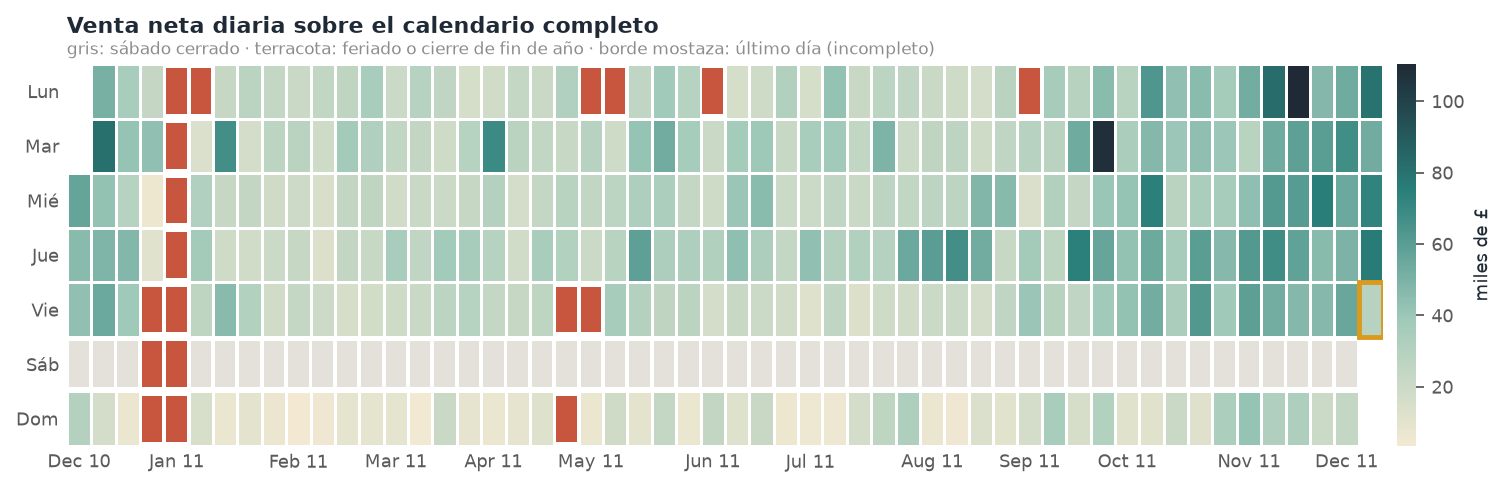
\includegraphics[width=\textwidth]{p2_calendario.png}
\caption{Venta neta diaria sobre el calendario. Cada cuadro es un día; la
fila de los sábados está completamente cerrada.}
\label{fig:calendario}
\end{figure}

\subsection{Los días sin transacciones (2.2)}

La tienda \textbf{no abre los sábados}: los \TotalSabados{} sábados del
periodo están vacíos y no hay ni un sábado con ventas. Los otros
\OtrosCerrados{} días cerrados (más dos sábados que coinciden con fiestas) se
clasificaron contra el calendario oficial de bank holidays de Inglaterra y
Gales de 2011 en la Tabla~\ref{tab:cerrados}.

\begin{table}[htbp]\centering\small
\caption{Días sin transacciones que no se explican sólo por ser sábado.}
\label{tab:cerrados}
\begin{tabular}{@{}l l l c@{}}
\toprule
Fecha & Día & Clasificación & ¿Móvil? \\
\midrule
\filas{tabla_p2_cerrados}
\bottomrule
\end{tabular}
\end{table}

Hay tres grupos. El primero es el \textbf{cierre de fin de año}, del 24 de
diciembre al 3 de enero: incluye los días sustitutos de Navidad, Boxing Day
y Año Nuevo (los tres cayeron en fin de semana en 2010--2011, así que el
feriado se corrió al lunes o martes siguiente) y además la tienda no abrió
los días hábiles intermedios. El segundo son los \textbf{bank holidays}
normales: Viernes Santo, Lunes de Pascua y los tres lunes de mayo y agosto.
El tercero es el que no se repite: el \textbf{viernes 29 de abril de 2011},
feriado nacional por la boda real del príncipe Guillermo. Todo cierre queda
explicado; no hay ningún día faltante sin razón.

\begin{respuesta}
\textbf{¿Cuáles son móviles?} Los que dependen de la Pascua: el Viernes
Santo, el Domingo de Pascua (que no es bank holiday, pero la tienda no abrió
ese domingo) y el Lunes de Pascua. En 2011 cayeron del 22 al 25 de abril; en
2012 caen del 6 al 9. Por eso FPP2 dice que son de lo más difícil de modelar:
un indicador de ``abril'' o de ``semana 16'' no los captura. Los tres bank
holidays de mayo y agosto cambian de fecha, pero siempre caen en lunes, así
que no confunden el patrón semanal. La boda real ni siquiera es móvil: es
única, y ningún modelo la puede aprender de la historia.
\end{respuesta}

\subsection{¿Cero o faltante? (2.3)}

Depende de para qué se use la serie. Un día cerrado es \textbf{cero} cuando
la pregunta es contable: por ejemplo, la venta total de abril, el flujo de
caja de una semana o la media móvil de la Parte 3, que debe repartir la
venta de una semana entre sus siete días. Ese día de verdad entraron cero
libras. En cambio, es \textbf{faltante} cuando la pregunta es sobre el
comportamiento de la demanda en los días que se puede vender. Por ejemplo,
para estimar la venta promedio de un lunes, para calcular la ACF o para
ajustar un modelo, un día cerrado no es una observación del proceso: nadie
pudo comprar. Si se trata como cero, el modelo ve una caída de demanda que no
existió, y además la ACF se llena de ceros que producen una correlación
artificial cada siete días.

\subsection{El último día (2.4)}

El 9 de diciembre de 2011 \textbf{no está completo}. La última factura es de
las \UltimaHora, cuando la mediana de la hora de la última factura en el resto
de los días es \HoraCierreMediana. Ese día suma \VentaUltimoDia, frente a un
promedio de \VentaViernesPrevios{} en los ocho viernes anteriores, y además
contiene el par de 80\,995 unidades de la sección~\ref{sec:top6}. Es el
momento en que se extrajeron los datos, no el cierre del día. Por eso
\textbf{se descarta}: tomarlo como un viernes normal metería una caída
falsa justo al final de la serie, que es lo que más pesa en un pronóstico.

De aquí en adelante, la serie de trabajo es la diaria sobre el calendario
completo, con los días cerrados como faltantes y sin el 9 de diciembre.

% ===========================================================================
\newpage
\section{Parte 3: Tendencia, estacionalidad y autocorrelación}

\subsection{Tendencia (3.1)}

La tendencia se estima con una media móvil centrada de 7 días sobre el
calendario completo, con los días cerrados como cero
(figura~\ref{fig:tendencia}).

\begin{figure}[htbp]\centering
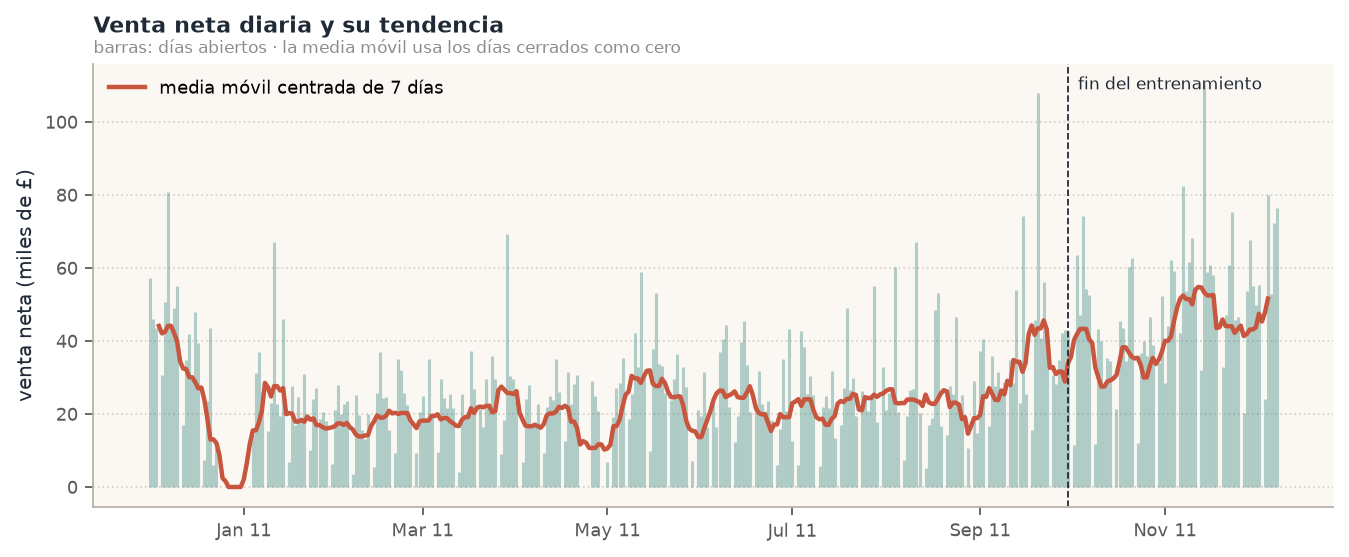
\includegraphics[width=\textwidth]{p3_tendencia.png}
\caption{Venta neta de los días abiertos (barras) y media móvil centrada de
7 días (línea).}
\label{fig:tendencia}
\end{figure}

\paragraph{¿Por qué 7?} Porque el patrón semanal se repite cada 7 días, y una
ventana de exactamente 7 días contiene una semana completa: cada día de la
semana entra una sola vez, así que el patrón semanal se cancela y lo que
queda es el nivel. Con 5 días la ventana contiene sólo parte de la semana, y
según dónde caiga incluye o no al sábado cerrado y al domingo flojo: la
``tendencia'' subiría y bajaría con el patrón semanal. Con 30 días el patrón
se cancela casi por completo, pero se borran cambios de nivel reales de pocas
semanas, como la caída de Navidad o el arranque de septiembre. Además, 30 no
es múltiplo de 7, así que cada ventana tiene un número distinto de cada día
de la semana.

\paragraph{¿Por qué centrada?} Para que el valor en $t$ represente el nivel
alrededor de $t$: usa tres días antes, el propio día y tres días después. Una
media móvil hacia atrás describe el nivel de hace tres días y llega tarde a
cada cambio. Para describir la serie eso no conviene, aunque, como se va a
ver en la Parte 5, para pronosticar es justo lo que no se puede usar.

\paragraph{La tendencia} Arranca alta en diciembre de 2010, se desploma a cero
con el cierre de fin de año y entre enero y agosto se mantiene bastante
estable, con un promedio de \MMEnero{} diarios. A partir de septiembre sube
con claridad y en noviembre promedia \MMNoviembre, con un máximo de
\MMMax: es la temporada en que los mayoristas se abastecen para Navidad. La
consecuencia para el resto de la tarea es que el periodo de prueba, de
octubre a diciembre, está en un nivel que el entrenamiento casi no conoce.

\subsection{Estacionalidad (3.2)}

Con el entrenamiento, para cada día abierto se calcula el cociente
$y_t/MA_t$ y el índice de cada día de la semana es el promedio de esos
cocientes (Tabla~\ref{tab:indices} y figura~\ref{fig:indices}).

\begin{table}[htbp]\centering\small
\caption{Índice estacional por día de la semana (entrenamiento).}
\label{tab:indices}
\begin{tabular}{@{}l r r@{}}
\toprule
Día & Índice & Días promediados \\
\midrule
\filas{tabla_p3_indices}
\bottomrule
\end{tabular}
\end{table}

\begin{figure}[htbp]\centering
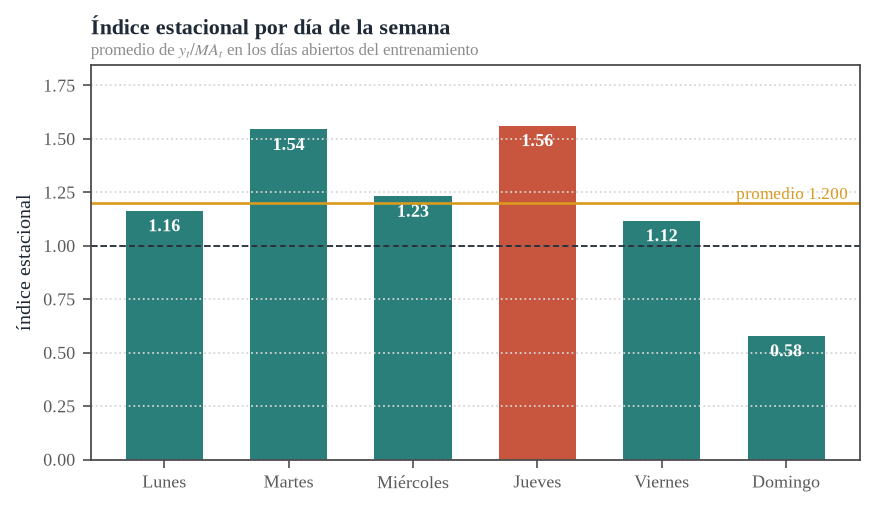
\includegraphics[width=0.66\textwidth]{p3_indices.png}
\caption{Índices estacionales. La línea punteada es 1 y la línea mostaza es
el promedio de los seis índices.}
\label{fig:indices}
\end{figure}

Los días que más venden son el \textbf{jueves} y el \textbf{martes}, alrededor
de un 55\,\% por encima del nivel de la semana. El \textbf{domingo} es por
mucho el día más flojo: vende poco más de la mitad del nivel. Tiene sentido
para una tienda que le vende sobre todo a negocios, que hacen sus pedidos en
días hábiles.

\begin{respuesta}
\textbf{¿Por qué el promedio no es 1?} Porque la media móvil reparte la venta
de la semana entre 7 días, y uno de ellos (el sábado) siempre vale cero. Si
la venta de una semana es $V$, la media móvil es aproximadamente $V/7$, y los
seis días abiertos venden en promedio $V/6$, así que su índice promedio
tiende a $7/6\approx1.167$. Si se incluyera el sábado con índice cero, los
siete índices sí promediarían cerca de 1. Sale un poco más, \PromIndices,
porque las semanas con feriados tienen todavía más ceros en la ventana y eso
infla los cocientes de los días abiertos de esas semanas.
\end{respuesta}

\subsection{Autocorrelación (3.3)}

Se usa la misma función $r_k$ de la Parte 0, ahora sobre los
\NEntrena{} días abiertos del entrenamiento, una fila por día y sin
calendario (figura~\ref{fig:acf}).

\begin{figure}[htbp]\centering
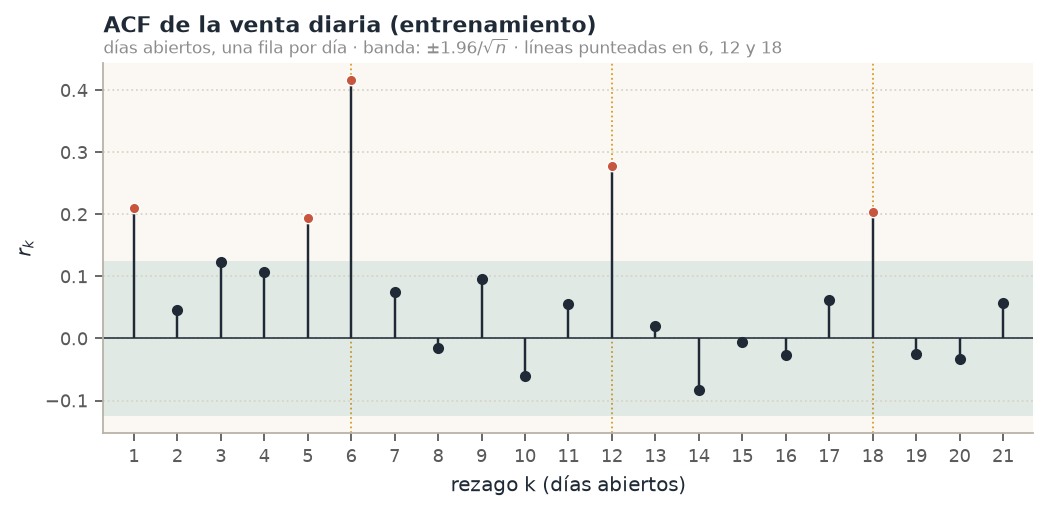
\includegraphics[width=0.85\textwidth]{p3_acf.png}
\caption{ACF de la venta en los días abiertos del entrenamiento. La banda es
$\pm1.96/\sqrt{\NEntrena}=\pm\BandaEntrena$.}
\label{fig:acf}
\end{figure}

\paragraph{(a)} Se salen de la banda \RezagosFuera{} de los 21 rezagos: el 1,
el 5, el 6, el 12 y el 18. La serie \textbf{no pasa} la prueba de retardo 1
de la Tarea 2: $r_1=\RunoReal$ es casi el doble de la banda. El pico está en
el \textbf{rezago \PicoACF} ($r_6=\RseisReal$), y se repite en 12 y 18. Seis
filas de días abiertos son, casi siempre, \textbf{7 días calendario}: una
semana completa, porque el sábado no tiene fila. Eso pasa en el
\SaltoSeisFrac{} de los casos; en el resto hay un feriado de por medio y la
distancia es de 8 días o más. Ljung--Box lo confirma sin ambigüedad:
$Q(6)=\QseisReal$ ($p=\PseisReal$) y $Q(12)=\QdoceReal$ ($p=\PdoceReal$).

\paragraph{(b)} La ACF mezcla las dos razones de la Parte 0. Los picos en 6,
12 y 18 se ven igual que el patrón semanal simulado en 0.4: es la media que
cambia según el día de la semana, no memoria. Los valores positivos en los
rezagos 1 al 5, que no caen rápido a cero, se parecen más a la tendencia
simulada. Eso es consistente con el cambio de nivel que se vio en 3.1, pero
también podría ser memoria genuina. Con esta gráfica no se puede separar una
cosa de la otra; para eso hay que quitar primero la estacionalidad, que es lo
que hace la Parte 4.

% ===========================================================================
\newpage
\section{Parte 4: Del AR(1) al SARIMA}

Toda esta parte trabaja con los \NEntrena{} días abiertos del entrenamiento
como una fila por día.

\subsection{Indicadoras de día de la semana (4.1)}

Se ajustó por OLS la venta contra seis variables indicadoras, una por día
abierto, sin intercepto. Cada coeficiente es simplemente la venta promedio de
ese día, y el residuo $e_t$ es cuánto se aleja cada día del promedio de su
día de la semana. La figura~\ref{fig:acfres} muestra la ACF de $e_t$ (panel
superior izquierdo) junto con las de los modelos siguientes, y la
Tabla~\ref{tab:lb4} reúne las pruebas de Ljung--Box de toda la parte.

\begin{figure}[htbp]\centering
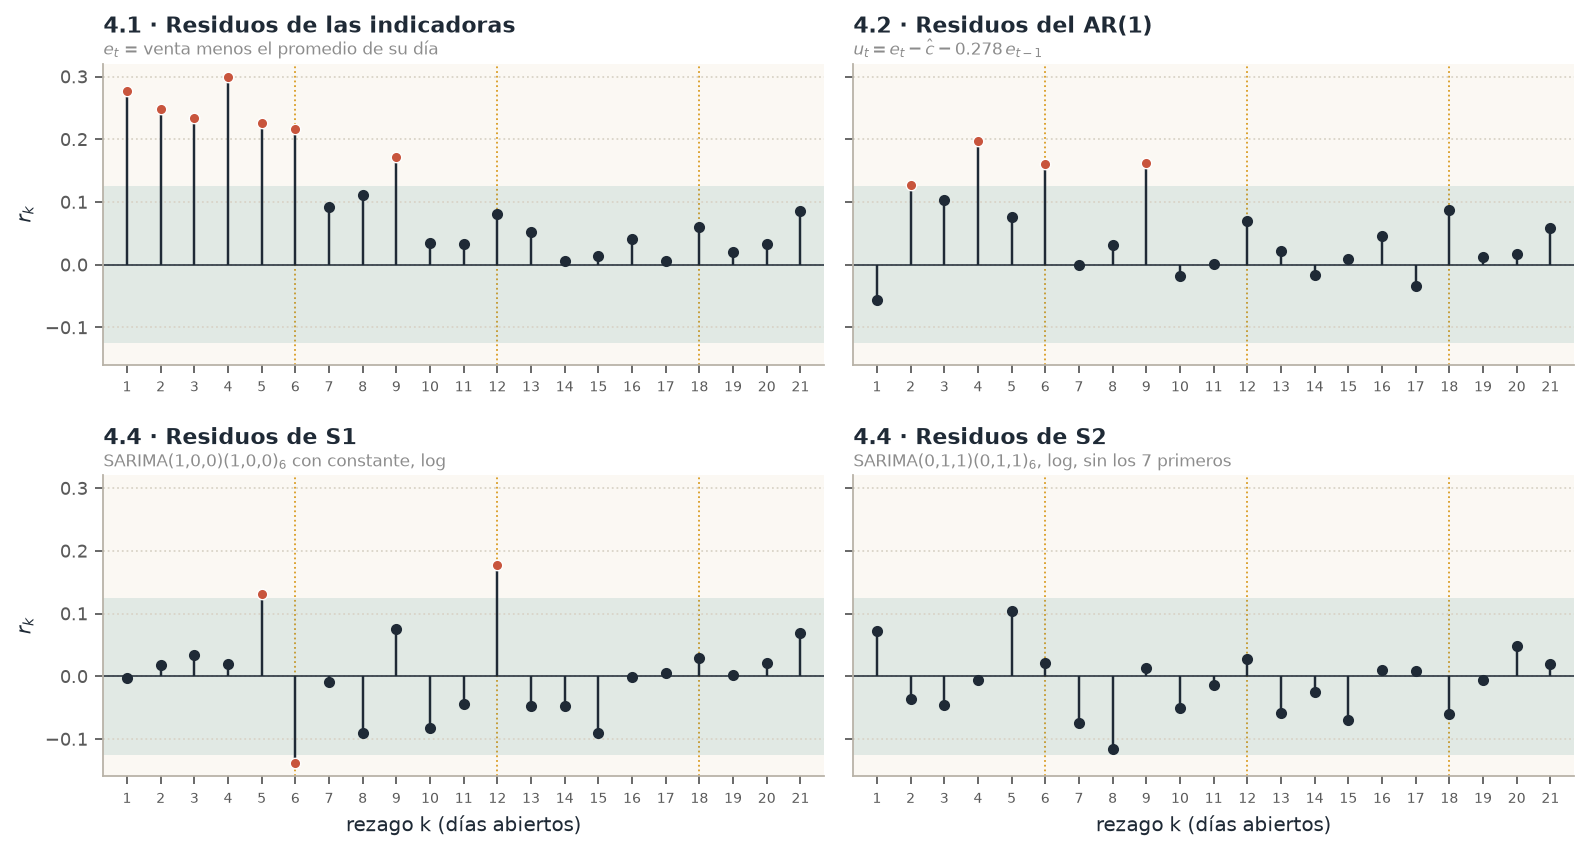
\includegraphics[width=\textwidth]{p4_acf_residuos.png}
\caption{ACF de los residuos de los cuatro modelos de la Parte 4. Las líneas
punteadas marcan los rezagos 6, 12 y 18.}
\label{fig:acfres}
\end{figure}

\begin{table}[htbp]\centering\small
\caption{Ljung--Box sobre los residuos de cada modelo. La última columna son
los grados de libertad usados para $Q(6)$ y $Q(12)$.}
\label{tab:lb4}
\begin{tabular}{@{}l r r r r c@{}}
\toprule
Residuos & $Q(6)$ & valor-$p$ & $Q(12)$ & valor-$p$ & g.\,l. \\
\midrule
\filas{tabla_p4_ljungbox}
\bottomrule
\end{tabular}
\end{table}

El pico estacional prácticamente desapareció: $r_{12}$ bajó de \RdoceReal{}
a \RedoceE{} y el patrón de 6, 12, 18 ya no domina. Pero quedó otra cosa:
los rezagos 1 a 6 están todos entre $0.2$ y $0.3$ y bajan muy despacio. Si
fuera un AR(1) con $\phi\approx\ReunoE$, la ACF tendría que caer como
$\phi^k$: $0.28$, $0.08$, $0.02$\ldots, y no es eso lo que se ve. La forma se
parece mucho más a la del proceso con tendencia de la Parte 0: una ACF casi
plana. Al modelo le falta \textbf{el nivel que cambia}. Las indicadoras
suponen que el lunes promedio es el mismo en enero que en septiembre, y los
residuos heredan todo el movimiento de la tendencia: semanas enteras quedan
por encima o por debajo de su promedio.

\subsection{AR(1) sobre los residuos (4.2)}

El OLS de $e_t$ contra $e_{t-1}$ da $\hat\phi=\PhiResiduos$. Con sus
residuos, $u_t = e_t-\hat c-\hat\phi\,e_{t-1}$, la ACF baja (panel superior
derecho), pero \textbf{todavía no parece ruido blanco}: siguen fuera de la
banda los rezagos \FueraU. Ljung--Box, con un grado de libertad menos por
haber estimado $\phi$, rechaza con claridad tanto con $m=6$ como con $m=12$.

\begin{respuesta}
\textbf{No alcanzó un AR(1).} Un AR(1) modela una memoria que se olvida
geométricamente, y lo que había en $e_t$ era en gran parte un nivel que se
mueve despacio. Un solo rezago no puede reproducir una ACF casi plana, y de
paso la correlación en el rezago 6 sigue ahí, porque el patrón semanal
tampoco es exactamente constante.
\end{respuesta}

\subsection{SARIMA (4.3)}

Lo anterior motiva modelos que combinen memoria de corto plazo, memoria
estacional y, si hace falta, diferencias para seguir un nivel que se mueve.
Con \code{SARIMAX} de statsmodels se ajustaron dos modelos sobre el logaritmo
de la venta, pasando el arreglo de valores sin fechas (porque las fechas
tienen huecos):
\begin{itemize}[leftmargin=1.2em]
\item \textbf{S1}: SARIMA$(1,0,0)(1,0,0)_6$ con constante. Es un AR(1) más
un AR estacional: hoy depende de ayer y del mismo día de la semana pasada.
Es estacionario.
\item \textbf{S2}: SARIMA$(0,1,1)(0,1,1)_6$ sin constante, el modelo de
aerolínea. Diferencia una vez y diferencia estacionalmente una vez, y corrige
con los errores recientes. No es estacionario.
\end{itemize}

\paragraph{¿Por qué $s=6$ y no 7?} Porque el modelo no ve fechas, ve filas, y
en las filas de días abiertos una semana tiene 6 días: el sábado no existe.
El mismo día de la semana pasada está 6 filas atrás, que es justo el pico
que se vio en 3.3. La suposición \textbf{se rompe en las semanas con
feriado}: si un lunes cierra, esa semana tiene 5 filas y, durante las
siguientes, ``6 filas atrás'' ya no es el mismo día de la semana sino el
anterior. En estos datos eso pasa en la Pascua, la boda real, los bank
holidays de lunes y, sobre todo, en las dos semanas del cierre de fin de año
(en total, en el 12\,\% de los saltos de 6 filas medidos en 3.3).

\paragraph{¿Por qué el logaritmo?} Porque la variación de la serie crece con
su nivel: en el otoño, cuando la venta es más alta, las diferencias entre
días también son más grandes. FPP2 recomienda transformar justo en ese caso.
En logaritmo, un efecto multiplicativo como ``el jueves vende 55\,\% más'' se
vuelve aditivo, que es lo que suponen los modelos ARIMA, y la varianza se
estabiliza. Además, todos los días abiertos tienen venta neta positiva, así
que el logaritmo existe.

\paragraph{Convergencia} La Tabla~\ref{tab:conv} compara el ajuste con las 50
iteraciones por defecto y con 500.

\begin{table}[htbp]\centering\small
\caption{Convergencia del optimizador. Los parámetros de S1 son
(\NombresSuno) y los de S2 son (\NombresSdos).}
\label{tab:conv}
\begin{tabular}{@{}l l c r l@{}}
\toprule
Modelo & \code{maxiter} & ¿Convergió? & Iteraciones & Parámetros \\
\midrule
\filas{tabla_p4_convergencia}
\bottomrule
\end{tabular}
\end{table}

S2 converge en 14 iteraciones y da lo mismo con cualquier límite. S1, en
cambio, \textbf{no converge} con el límite por defecto, y lo que devuelve en
ese caso es engañoso: el AR estacional queda en $0.895$ y la constante en
$0.937$. Con 500 iteraciones converge en 81, y el AR estacional baja a
$\SunoPhiS$ mientras la constante sube a $\SunoConst$. Los dos juegos de
parámetros dan una media parecida: en un AR la media es la constante dividida
entre $(1-\phi)(1-\Phi)$, así que el optimizador puede subir $\Phi$ y bajar la
constante casi sin cambiar el ajuste. Por eso le cuesta encontrar el óptimo.
Un $\Phi$ de $0.9$ implicaría una memoria estacional mucho más larga de la
que hay. En lo que sigue se usa siempre la versión que convergió.

\subsection{Diagnóstico (4.4)}

Los paneles inferiores de la figura~\ref{fig:acfres} y las dos últimas filas
de la Tabla~\ref{tab:lb4} muestran los residuos de los dos SARIMA, con
$m-2$ grados de libertad porque cada modelo estima dos coeficientes ARMA.
Para S2 se descartan los primeros 7 residuos, que son artefactos del arranque
de las diferencias.

\begin{respuesta}
\textbf{S2 deja residuos de ruido blanco y S1 no.} En S2 ningún rezago se
sale de la banda y Ljung--Box no rechaza ($p=0.30$ y $p=0.40$). En S1 se
salen los rezagos 5, 6 y 12, y Ljung--Box rechaza al 5\,\% con ambos $m$. El
patrón es el mismo que en 4.1: lo que S1 no captura es el nivel que se
mueve, y las diferencias de S2 son justamente la herramienta para eso.
\end{respuesta}

\subsection{¿Hacia dónde van los pronósticos? (4.5)}

S1 es estacionario, así que se comporta como el AR(1) de la Parte 0: el
efecto de lo último observado se olvida geométricamente. A medida que el
horizonte crece, sus pronósticos \textbf{regresan a la media del proceso},
que en libras es $\exp(c/((1-\phi)(1-\Phi)))\approx\MediaSuno$, y el patrón
semanal se va apagando como $\Phi^k$. S2 se parece a la caminata aleatoria:
nunca olvida. Sus pronósticos \textbf{no regresan a nada}: arrancan del
último nivel observado, repiten el patrón semanal reciente y, como tiene una
diferencia normal y una estacional, prolongan además la pendiente local que
traía la serie. Su incertidumbre también crece sin límite con el horizonte,
igual que $\Var(Y_t)=t\sigma^2$.

La figura~\ref{fig:horizonte} lo muestra con los dos modelos ajustados con
todo el entrenamiento. S1 se aplana enseguida en unas \MediaSuno, el nivel
de enero a agosto, mientras que S2 sigue la subida de septiembre. Esto ya
anticipa qué va a pasar en la Parte 5, cuando la venta de octubre a
diciembre esté muy por encima del nivel histórico.

\begin{figure}[htbp]\centering
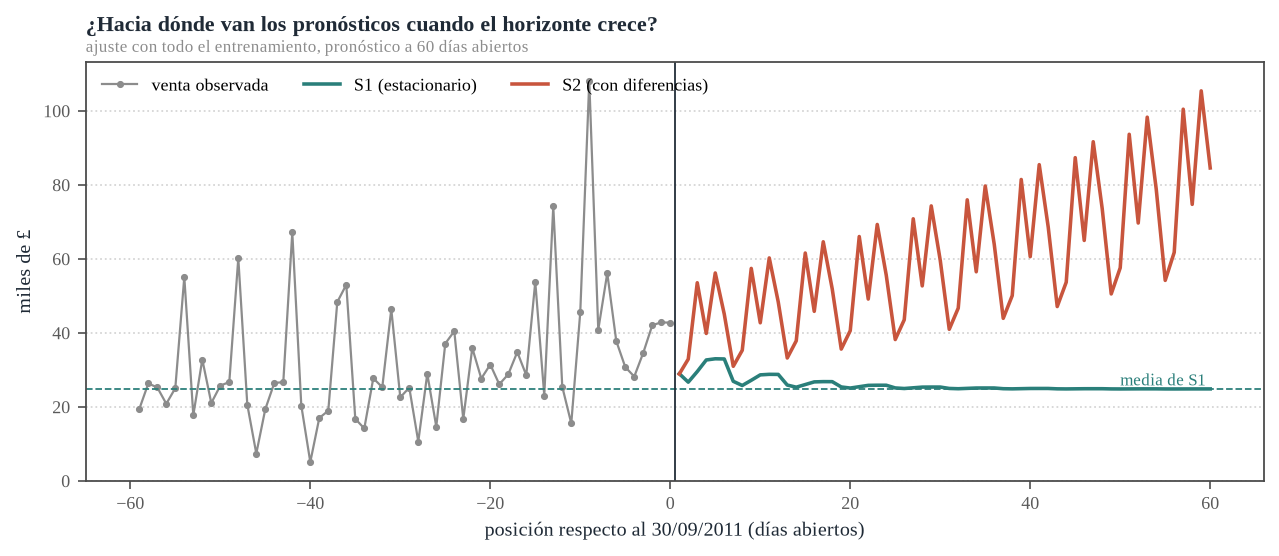
\includegraphics[width=0.92\textwidth]{p4_horizonte.png}
\caption{Pronósticos a 60 días abiertos desde el 30 de septiembre.}
\label{fig:horizonte}
\end{figure}

% ===========================================================================
\newpage
\section{Parte 5: Pronóstico y fuga}

El pronóstico se hace como en la vida real: cada domingo, con todo lo
observado hasta ese día (incluida la venta del domingo), se pronostican los
días abiertos de lunes a domingo siguientes. Después se avanza una semana, se
reajusta y se repite.

\subsection{Los seis modelos (5.1)}

Además de S1 y S2 se implementaron:
\begin{itemize}[leftmargin=1.2em]
\item \textbf{B1}: la media histórica de los días abiertos.
\item \textbf{B2}: el naive estacional, que pronostica el valor del mismo día
de la semana abierto más reciente.
\item \textbf{M1}: OLS con una tendencia lineal en $t$ (días desde el 1 de
diciembre de 2010) más las seis indicadoras.
\item \textbf{M2}: OLS con las seis indicadoras y dos rezagos, $y_{t-7}$ y
$y_{t-14}$. Si alguno cae en un día cerrado, se usa el mismo día de la
semana abierto más reciente; en la práctica, $y_{t-7}$ es el último día
abierto con el mismo día de la semana e $y_{t-14}$ el anterior a ése. Se
comprobó con el ejemplo del enunciado: para el 9 de mayo, $y_{t-7}$ vale
\LagMayo, que es la venta del 18 de abril. Las filas sin rezago al inicio de
la serie no se usan para ajustar.
\end{itemize}
Para S1 y S2, el horizonte de cada objetivo es su posición entre los días
abiertos posteriores al origen. Se usó la configuración que convergió en 4.3
y se verificó \code{mle\_retvals['converged']} en cada reajuste: S1 convergió
en \ConvSuno{} orígenes y S2 en \ConvSdos.

\begin{respuesta}
\textbf{¿Por qué M2 puede usar $y_{t-7}$ y no $y_{t-1}$?} Desde un domingo,
el día más lejano que se pronostica es el domingo siguiente, siete días
después. Para cualquier objetivo de esa semana, $t-7$ cae en el origen o
antes, así que $y_{t-7}$ ya se observó. Con $y_{t-1}$ sólo se podría
pronosticar el lunes: para el martes haría falta la venta del lunes, que
todavía no ocurrió. M2 es un modelo de un paso que no sabe pronosticar sus
propios predictores.

\textbf{¿Cómo usa S1 el rezago 1?} De forma recursiva. Para el lunes usa el
domingo observado; para el martes usa \emph{su propio pronóstico} del lunes
en lugar del valor real, y así sucesivamente. El modelo especifica cómo se
genera toda la serie, así que puede pronosticar sus propios rezagos, y el
filtro de Kalman de statsmodels lo hace automáticamente. El precio es que el
error se acumula con el horizonte.
\end{respuesta}

\subsection{Tres formas de estimar el error (5.2)}

La Tabla~\ref{tab:errores} reúne el MAE y el RMSE de los seis modelos
estimados de tres formas:
\begin{enumerate}[label=(\alph*), leftmargin=1.6em]
\item validación cruzada aleatoria de 5 folds sobre el entrenamiento, repetida
con 10 semillas (141903 a 141912); se reporta la media y la desviación
estándar entre semillas;
\item origen móvil semanal dentro del entrenamiento, con los \NorigenesB{}
domingos de mayo a septiembre como orígenes y \NdiasB{} días evaluados;
\item el periodo de prueba con origen móvil semanal: \NorigenesC{} orígenes,
del 2 de octubre al 4 de diciembre, y los \NdiasC{} días abiertos del 3 de
octubre al 8 de diciembre.
\end{enumerate}
En los tres casos el MAE y el RMSE se calculan juntando todos los días
pronosticados.

\begin{table}[htbp]\centering\small
\caption{MAE y RMSE en libras. (a) y (b) son dentro del entrenamiento. En (a), media $\pm$ desviación estándar entre
las 10 semillas.}
\label{tab:errores}
\setlength{\tabcolsep}{4.5pt}
\begin{tabular}{@{}l rr rr rr@{}}
\toprule
& \multicolumn{2}{c}{(a) CV aleatoria} & \multicolumn{2}{c}{(b) Origen móvil}
& \multicolumn{2}{c}{(c) Prueba} \\
\cmidrule(lr){2-3}\cmidrule(lr){4-5}\cmidrule(lr){6-7}
Modelo & MAE & RMSE & MAE & RMSE & MAE & RMSE \\
\midrule
\filas{tabla_p5_errores}
\bottomrule
\end{tabular}
\end{table}

\paragraph{¿Por qué (a) no tiene sentido para B2, S1 y S2?} Porque los tres
dependen del orden. B2 pronostica con ``el valor más reciente del mismo
día'', y en un fold aleatorio lo más reciente puede ser un día posterior al
que se pronostica. S1 y S2 necesitan la serie como una secuencia contigua
para calcular sus rezagos y diferencias; si se le quitan días al azar, la
fila anterior ya no es el día anterior, y no queda claro ni qué se está
ajustando. En general, la validación cruzada aleatoria usa el futuro para
pronosticar el pasado, que es justo lo que en series de tiempo no se puede
hacer.

\paragraph{¿Cuál se acerca más a (c)?} La (b). Para los tres modelos que
tienen las tres estimaciones, (a) da el error más bajo, (b) uno un poco más
alto y (c) el más alto de todos: para M2, \MAEaMdos{}{}, \MAEbMdos{}{} y \MAEcMdos{}. La
validación aleatoria es optimista porque cada día de prueba tiene vecinos de
ambos lados en el entrenamiento. Pero \textbf{ninguna se acerca de verdad}:
en prueba, el MAE es entre 1.25 y 1.7 veces lo que prometía
(b), y para B1 más del doble. El ranking de los modelos también cambia: en
(b) gana M2 y S2 queda en medio de la tabla; en (c) S2 es el mejor.

\subsection{¿Qué modelo gana en prueba? (5.3)}

\textbf{Gana \Ganador}, con un MAE de \pounds\MAEcSdos{}, seguido de B2
(\pounds\MAEcBdos{}). La figura~\ref{fig:prueba} muestra por qué.

\begin{figure}[htbp]\centering
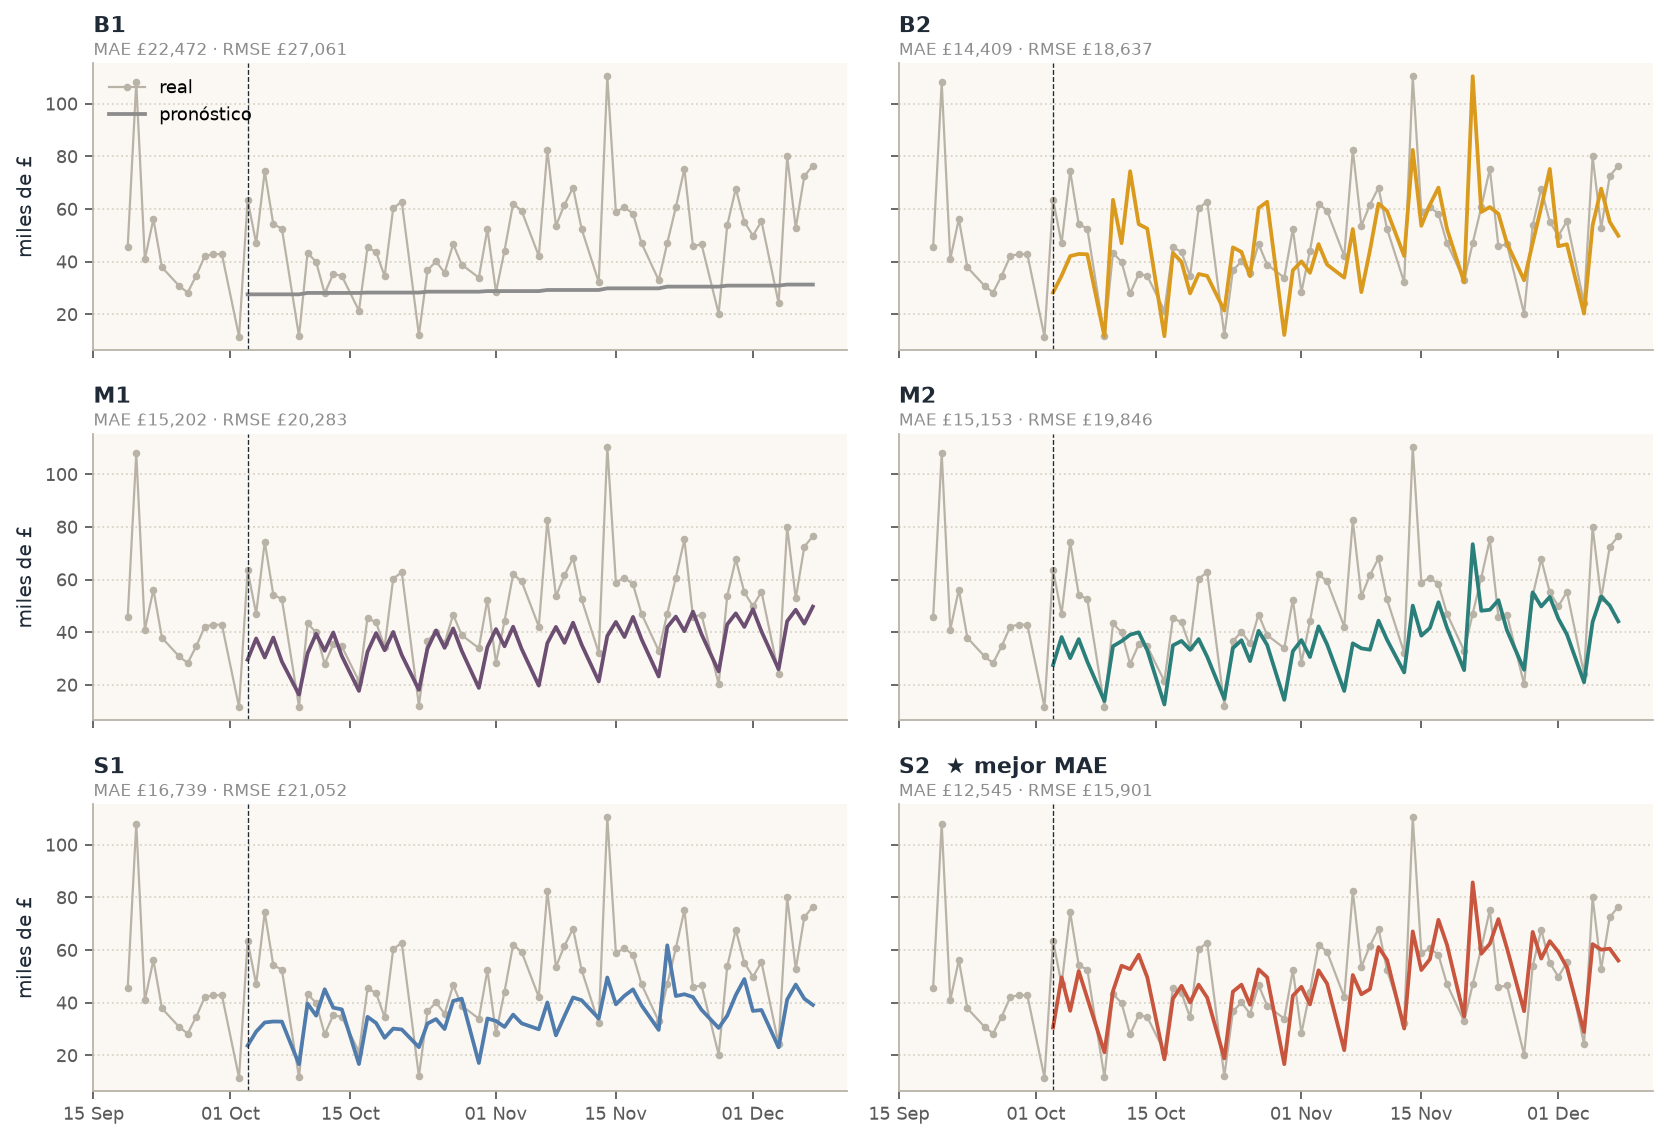
\includegraphics[width=\textwidth]{p5_prueba.png}
\caption{Pronósticos semanales con origen móvil (en color) contra la venta
real (en gris) en el periodo de prueba. La línea punteada marca el 3 de
octubre.}
\label{fig:prueba}
\end{figure}

En el periodo de prueba la venta promedio por día abierto fue de
\MediaPrueba, contra \MediaEntrena{} en el entrenamiento. Los modelos que
están anclados a la historia completa se quedan abajo todo el periodo: B1
pronostica una línea casi plana alrededor de la media histórica, S1 regresa
a su media de unas \MediaSuno{} (como se anticipó en 4.5), y M1 y M2 suben un
poco con la tendencia y los rezagos, pero se quedan cortos. Los dos modelos
que mejor siguen la subida son los que arrancan cada semana del nivel más
reciente: B2, que repite la semana anterior, y S2, que además la suaviza. B2
copia todo, incluido el ruido: un día atípico se repite la semana siguiente
(se ve a fines de noviembre, cuando repite el pico de la semana anterior). S2, en cambio, promedia el
pasado reciente a través de sus términos MA, así que se mueve con el nivel
sin copiar cada sobresalto. Eso coincide con el diagnóstico de 4.4: S2 era
el único modelo cuyos residuos parecían ruido blanco, o sea, el único que
había capturado la estructura completa de la serie, incluido el nivel que
cambia.

\subsection{La trampa (5.4)}

Un compañero propone agregarle a M2 la media móvil centrada de 7 días de la
Parte 3 como predictor. Con la media móvil calculada una sola vez sobre toda
la serie, el resultado está en la última fila de la Tabla~\ref{tab:errores}:
en (a) el MAE baja de \MAEaMdos{}{} a \MAEaTrampa{} y en (b) de \MAEbMdos{}{} a
\MAEbTrampa. Se ve mejor que cualquier otro modelo.

\begin{respuesta}
\textbf{Por qué es ilegal.} La media móvil centrada en $t$ promedia
$y_{t-3},\dots,y_{t+3}$. Incluye la venta del propio día que se quiere
pronosticar y tres días del futuro. En la vida real, el domingo en que se
hace el pronóstico nadie conoce esos valores. El modelo no aprendió a
pronosticar: aprendió a leer una versión suavizada de la respuesta.

\textbf{Por qué el origen móvil no lo detecta.} El origen móvil respeta el
tiempo en las \emph{filas}: sólo ajusta con días anteriores al origen. Pero
la columna de la media móvil se calculó una vez, con toda la serie, antes de
partir nada. Cuando el procedimiento lee el predictor de un día objetivo,
ese número ya contiene la venta de ese día y de los tres siguientes. La fuga
está en la construcción de la variable, no en la partición, y ninguna
partición la puede ver.

\textbf{Por qué (c) no se puede calcular sin trampa.} Para pronosticar el
jueves 8 de diciembre con este modelo hace falta la media móvil de ese día,
que necesita las ventas del 5 al 11 de diciembre: el valor que se quiere
pronosticar y días que ni siquiera están en los datos. Para cualquier día de
prueba, calcular el predictor exige usar justo los datos de prueba que se
supone que no se conocen. Lo único honesto sería sustituirla por una media
móvil hacia atrás, que ya es otro modelo.
\end{respuesta}

\subsection{¿Por qué todo se queda corto? (5.5)}

Hay dos causas distintas.

La primera viene de \textbf{cómo se partieron los datos}. La validación
cruzada aleatoria mezcla pasado y futuro: cada día de prueba tiene vecinos
de ambos lados en el entrenamiento, y los modelos con rezagos (como M2) ven
en el entrenamiento días posteriores a los que pronostican. Por eso (a) es
el más optimista. Esta causa \textbf{sí se arregla} con una mejor validación:
el origen móvil reproduce exactamente las condiciones del pronóstico real, y
por eso (b) da errores más grandes que (a).

La segunda es que \textbf{la serie cambió}. De octubre a diciembre la tienda
vendió casi el doble por día que en el resto del año, y con el nivel crecen
también los errores. Cualquier validación hecha dentro del entrenamiento
mide el error en un régimen de enero a septiembre que ya no es el de la
prueba. Esta causa \textbf{no se arregla} con una mejor validación: el
origen móvil (b) también se quedó corto, porque no hay ninguna forma de
medir dentro del entrenamiento el error de un periodo que el entrenamiento
nunca vio.

\begin{respuesta}
\textbf{¿Se puede estimar la estacionalidad anual con un año de datos?} No.
Para estimar un efecto estacional hay que ver el mismo momento del ciclo
varias veces y promediar. Con un solo año, cada mes aparece una vez (y
diciembre, a medias, dos), así que no hay forma de separar ``noviembre
siempre es alto'' de ``la tienda está creciendo'' o de ``este noviembre fue
especial''. La estacionalidad anual y la tendencia quedan confundidas. Se
necesitan al menos dos o tres años completos. Ésa es exactamente la parte
de la serie que hizo fallar a todos los modelos en la prueba.
\end{respuesta}

% ===========================================================================
\newpage
\section{Parte 6: Detrás de la serie hay clientes: análisis RFM}

\subsection{R, F y M al 1 de octubre (6.1)}

Con los datos limpios que tienen \code{CustomerID} y sólo las transacciones
anteriores al 1 de octubre de 2011, para cada cliente se calculó:
\begin{itemize}[leftmargin=1.2em]
\item \textbf{R}: los días entre su última factura de venta y el 1 de octubre;
\item \textbf{F}: el número de facturas de venta distintas (las cancelaciones
no cuentan como compras);
\item \textbf{M}: la venta neta total, cancelaciones incluidas.
\end{itemize}

Hay \textbf{\ClientesRFM{} clientes} con al menos una factura de venta antes
del 1 de octubre. Otros \ClientesSoloCancel{} identificadores sólo tienen
cancelaciones en ese periodo (devoluciones de compras anteriores a diciembre
de 2010, que no están en el archivo). No tienen una compra a partir de la
cual medir la recencia, así que no entran.

\ClientesMneg{} clientes tienen \textbf{$M\le0$}: devolvieron tanto o más de
lo que compraron, como el cliente 12346 de la sección~\ref{sec:top6}. Se
dejan en el análisis, porque el enunciado pide puntuarlos junto con los
demás. Su puntaje de monto queda en 1 de forma natural, que es lo correcto:
en términos netos no le han dejado dinero a la tienda.

\begin{respuesta}
\textbf{¿Por qué no usar nada posterior al 1 de octubre?} Porque en 6.3 se
va a medir qué tan bien RFM anticipa quién compra después de esa fecha. Si R,
F o M incluyeran transacciones posteriores, un cliente que compró en
noviembre tendría recencia corta \emph{porque} compró en noviembre, y el
análisis se estaría prediciendo a sí mismo. Es la misma fuga de la Parte
5.4, ahora con clientes en lugar de días.
\end{respuesta}

\subsection{Puntajes por quintiles (6.2)}

Cada dimensión se convierte en un puntaje de 1 a 5 por quintiles, con 5 como
lo mejor: la recencia más corta, la frecuencia más alta y el monto más alto.

\textbf{El problema con F} es que es un conteo con muchísimos empates: el
\FracFuno{} de los clientes tiene $F=1$. El primer quintil termina en $F=1$,
pero también el segundo, así que los bordes de los quintiles se repiten y
\code{pd.qcut} directamente sobre F falla. No hay manera de partir a los
clientes en cinco grupos del mismo tamaño usando sólo el valor de F.

Para que el resultado sea reproducible se siguió el procedimiento del
enunciado: los clientes ordenados por \code{CustomerID}, barajados con
\code{numpy.random.default\_rng(2026).permutation}, y después
\code{pd.qcut(F.rank(method='first'), 5)}. Se usó el mismo orden barajado
para R y M, que también tienen empates (muchos clientes compraron por última
vez el mismo día).

\begin{respuesta}
\textbf{¿Qué implica para dos clientes con la misma F?} Que pueden terminar
con puntajes distintos sólo por suerte. Los clientes con $F=1$ quedan
repartidos entre los puntajes 1, 2 y 3 según el orden en que los dejó la
permutación. Entre ellos, la diferencia de puntaje no significa nada: con
otra semilla un cliente con puntaje 3 podría tener 1. El puntaje es
reproducible, pero en los empates no es informativo, y conviene tenerlo en
cuenta antes de tratar a un cliente con $F_s=3$ como más valioso que otro con
$F_s=1$.
\end{respuesta}

\subsection{¿Quién vuelve a comprar? (6.3)}

Sea $\text{compra}_i=1$ si el cliente tiene al menos una factura de venta
entre el 1 de octubre y el 8 de diciembre. Lo cumple el \FracCompra{} de los
clientes. La Tabla~\ref{tab:tasas} y la figura~\ref{fig:tasas} muestran la
fracción que compró para cada puntaje, y la Tabla~\ref{tab:auc} da el AUC de
cada dimensión como clasificador de $\text{compra}_i$, con los valores crudos
(R con el signo invertido, para que más alto sea mejor).

\begin{table}[htbp]\centering\small
\begin{minipage}{0.46\textwidth}\centering
\caption{Fracción que compró, por puntaje.}
\label{tab:tasas}
\begin{tabular}{@{}c r r r@{}}
\toprule
Puntaje & R & F & M \\
\midrule
\filas{tabla_p6_tasas}
\bottomrule
\end{tabular}
\end{minipage}\hfill
\begin{minipage}{0.5\textwidth}\centering
\caption{AUC como clasificador de $\text{compra}_i$.}
\label{tab:auc}
\begin{tabular}{@{}l r r r r@{}}
\toprule
& $-$R & F & M & $R_s+F_s+M_s$ \\
\midrule
\filas{tabla_p6_auc}
\bottomrule
\end{tabular}
\end{minipage}
\end{table}

\begin{figure}[htbp]\centering
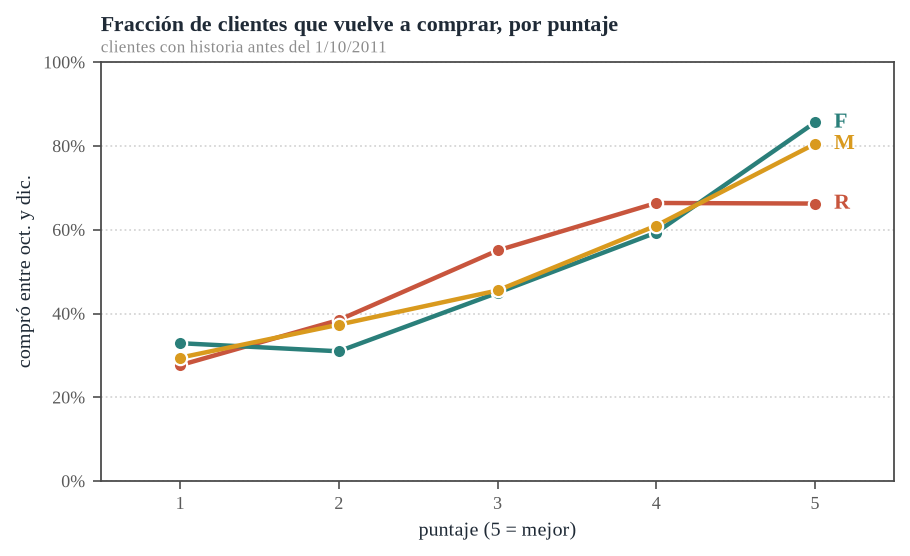
\includegraphics[width=0.68\textwidth]{p6_tasas.png}
\caption{Fracción de clientes que volvió a comprar entre octubre y
diciembre, para cada puntaje de R, F y M.}
\label{fig:tasas}
\end{figure}

Las tres dimensiones separan en la dirección esperada: a mejor puntaje, más
probable que el cliente vuelva. \textbf{F es la que mejor separa}: del
puntaje 1 al 5 la tasa pasa de 33\,\% a 86\,\%, y tiene el AUC individual más
alto (\AUCF). Lo plano entre los puntajes 1 y 2 de F es justamente el efecto
del desempate al azar: los dos grupos son clientes con $F=1$, así que en
realidad no hay diferencia entre ellos. M queda muy cerca (\AUCM), lo cual es
natural porque quien compra seguido acumula más monto. R es la más débil
(\AUCR), y su curva se aplana arriba: los puntajes 4 y 5 compran en la misma
proporción. Haber comprado hace dos semanas o hace dos meses importa poco
para un mayorista que pide con cierta periodicidad. La suma de los tres
puntajes le gana a cada uno por separado (\AUCSuma), pero por poco: las tres
dimensiones están muy correlacionadas y se repiten bastante información.

\subsection{Los campeones (6.4)}

Los ``campeones'' son los clientes con puntaje 4 o 5 en las tres
dimensiones. Son \NCampeones{} clientes, el \textbf{\FracCampeones} del
total, y generaron el \textbf{\VentaCampeones} de la venta neta del 1 de
octubre al 8 de diciembre de todos los clientes con \code{CustomerID}
(\VentaOctDic), incluidos los nuevos (figura~\ref{fig:reparto}). Es la
concentración típica de este tipo de negocio: una quinta parte de los
clientes hace más de la mitad de la venta.

\begin{figure}[htbp]\centering
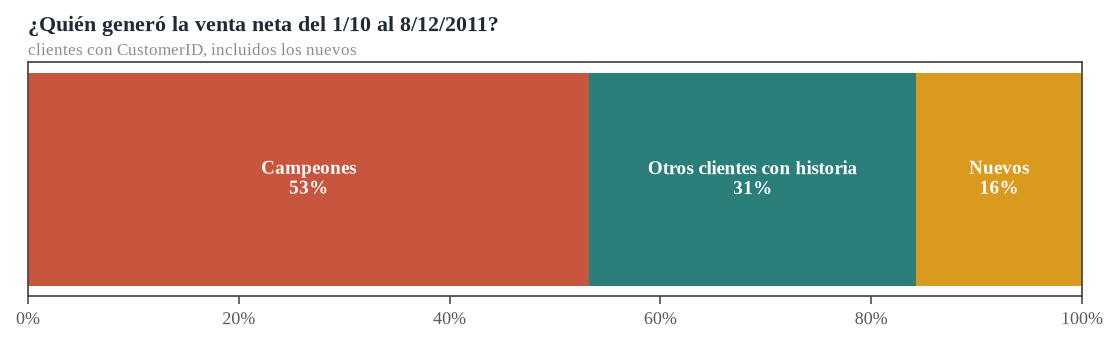
\includegraphics[width=0.85\textwidth]{p6_reparto.png}
\caption{Reparto de la venta neta del 1 de octubre al 8 de diciembre entre
campeones, el resto de los clientes con historia y los clientes nuevos.}
\label{fig:reparto}
\end{figure}

\subsection{Los clientes nuevos (6.5)}

Los clientes nuevos, los que no tenían ninguna factura de venta antes del 1
de octubre, fueron \NNuevos{} y generaron el \textbf{\VentaNuevos} de la
venta neta de octubre a diciembre de los clientes con \code{CustomerID}.

\begin{respuesta}
\textbf{¿Puede RFM, o un modelo cliente por cliente, pronosticar esa venta?}
No. RFM, y cualquier modelo que se construya cliente por cliente, sólo puede
puntuar o pronosticar a los clientes que ya existen en la historia: un
cliente nuevo no tiene R, ni F, ni M, ni fila en la tabla. Si se pronostica
cada cliente y se suma (\emph{bottom-up}), ese \VentaNuevos{} no aparece en
ningún lado, y el total queda sistemáticamente corto. En cambio, la serie
agregada de la Parte 5 (\emph{top-down}) sí incluye a los clientes nuevos: no
sabe quiénes son, pero su venta está dentro de cada día del total, así que
la tendencia que siguieron B2 y S2 en otoño ya incluye a los clientes que
llegaron en esa temporada.

\textbf{Conexión con el proyecto.} En el proyecto se va a comparar un
pronóstico construido cliente por cliente contra uno sobre la serie
agregada. Este resultado dice que el \emph{bottom-up} parte con una
desventaja estructural de alrededor de un 16\,\% en esta época del año, a
menos que se le agregue un componente aparte para la llegada de clientes
nuevos. A cambio, el enfoque por cliente sabe \emph{quién} va a comprar, que
el agregado no puede saber.
\end{respuesta}

% ===========================================================================
\newpage
\section{Conclusiones}

\begin{itemize}[leftmargin=1.2em]
\item Una serie puede reprobar una prueba de independencia por memoria o por
una media que cambia, y las dos cosas se ven distinto en la ACF: la memoria
del AR(1) cae como $\phi^k$, mientras que una tendencia deja una ACF casi
plana y una estacionalidad deja picos en el periodo. La prueba de retardo 1
reprobó a una tendencia sin memoria y dejó pasar un patrón semanal, el mismo
error de diseño que dejó pasar a RANDU en la Tarea 2. Ljung--Box sólo lo
arregla si $m$ cubre el periodo estacional.
\item El estimador OLS del AR(1) tiene un sesgo hacia abajo de orden $1/n$
que crece al acercarse a la raíz unitaria, y para la caminata aleatoria
$r_k$ no estima nada que exista.
\item En los datos reales, la limpieza movió poco dinero en total, pero las
decisiones importan: conservar las líneas Manual es lo que permite que la
venta mal capturada de las canastas se cancele al netear por día. Las seis
líneas más grandes del archivo resultaron ser tres errores corregidos el
mismo día.
\item El calendario explica todos los días faltantes: sábados, el cierre de
fin de año, la Pascua, los bank holidays y la boda real. Al trabajar con
filas de días abiertos, la semana mide 6 filas, y de ahí sale $s=6$.
\item La autocorrelación de la venta es una mezcla de estacionalidad semanal
y de un nivel que se mueve. Quitar el día de la semana no basta, y un AR(1)
tampoco; el modelo con diferencias S2 es el único que deja residuos de ruido
blanco.
\item S2 ganó en prueba, pero todas las estimaciones dentro del entrenamiento
se quedaron cortas. Parte de eso se arregla validando con origen móvil en
lugar de folds aleatorios; la otra parte, que la serie casi duplicó su nivel
en la temporada navideña, no se puede arreglar con un año de datos. Un
predictor que mira el futuro, como la media móvil centrada, hace que el
modelo se vea mejor y ninguna partición lo detecta.
\item Detrás de la serie, una quinta parte de los clientes hace más de la
mitad de la venta, y los clientes nuevos aportan cerca de una sexta parte
que sólo el pronóstico agregado puede ver.
\end{itemize}

% ===========================================================================
\begin{thebibliography}{9}
\bibitem{chen15} D. Chen. \emph{Online Retail} [conjunto de datos]. UCI
Machine Learning Repository, 2015.
\url{https://archive.ics.uci.edu/dataset/352/online+retail}
\bibitem{chen12} D. Chen, S. L. Sain y K. Guo. Data mining for the online
retail industry: A case study of RFM model-based customer segmentation using
data mining. \emph{Journal of Database Marketing \& Customer Strategy
Management}, 19(3):197--208, 2012.
\bibitem{fpp2} R. J. Hyndman y G. Athanasopoulos. \emph{Forecasting:
Principles and Practice}, 2a ed. OTexts, Melbourne, 2018.
\url{https://otexts.com/fpp2/}
\bibitem{tsay} R. S. Tsay. \emph{Analysis of Financial Time Series}, 2a ed.
Wiley, 2005.
\bibitem{govuk} Gobierno del Reino Unido. \emph{UK bank holidays}.
\url{https://www.gov.uk/bank-holidays}
\end{thebibliography}

\end{document}
